%-----------------------------------------------------------------------------%
\chapter{\babEmpat}
%-----------------------------------------------------------------------------%
Bab ini membahas proses pengujian dan evaluasi yang dilakukan terhadap sistem yang telah dikembangkan pada bab-bab sebelumnya. Pengujian dilakukan untuk memastikan bahwa setiap fitur berjalan sesuai dengan kebutuhan fungsional, standar kualitas, serta tujuan dari pembangunan sistem.

%-----------------------------------------------------------------------------%
\section{Tujuan Pengujian}
Tujuan dari pengujian ini adalah untuk memverifikasi fungsionalitas sistem, memvalidasi kesesuaian sistem dengan kebutuhan yang telah ditetapkan, serta menilai kualitas dan performa website secara keseluruhan.

\section{Lingkup Pengujian}
Bagian ini menjelaskan ruang lingkup pengujian yang dilakukan terhadap sistem, mencakup pengujian performa halaman, pengujian basis data, serta pengujian view. Setiap aspek diuji untuk memastikan bahwa sistem berfungsi sesuai kebutuhan, efisien, dan dapat memberikan pengalaman pengguna yang optimal.
\subsection{Pengujian Performa Halaman dengan Lighthouse Insights}
Pengujian performa website dilakukan menggunakan Lighthouse Insights untuk mendapatkan informasi mengenai kecepatan, efisiensi pemuatan halaman, serta identifikasi aspek-aspek teknis yang dapat dioptimalkan. Alat ini memberikan penilaian menyeluruh baik untuk tampilan mobile maupun desktop, termasuk metrik seperti Largest Contentful Paint (LCP), First Input Delay (FID), dan Cumulative Layout Shift (CLS).
\subsection{Pengujian Basis Data}
Pengujian basis data dilakukan untuk memastikan bahwa struktur tabel, integritas data, serta operasi CRUD pada setiap model bekerja sesuai dengan rancangan sistem. Pada tahap ini, pengujian dilakukan menggunakan pytest dan Django ORM untuk memverifikasi bahwa setiap entitas dapat dibuat, dibaca, diperbarui, dan dihapus dengan benar tanpa menimbulkan inkonsistensi data.
\subsection{Pengujian View}
Pengujian view pada Django dilakukan untuk memastikan bahwa setiap halaman dalam sistem bekerja sesuai fungsinya. Fokus utama dari pengujian ini adalah memverifikasi bahwa seluruh URL dapat diakses, setiap view memberikan respons yang benar (seperti status code 200 atau 302).

\section{Metode Pengujian}

Metode pengujian yang digunakan dalam sistem ini bertujuan untuk memastikan bahwa seluruh komponen aplikasi bekerja sesuai dengan kebutuhan fungsional maupun non-fungsional. Pengujian dilakukan menggunakan pendekatan \textit{black-box testing} untuk memvalidasi keluaran berdasarkan input tanpa melihat implementasi internal. Selain itu, beberapa alat bantu seperti Lighthouse Insights, \texttt{pytest}, dan \textit{Django Test Client} digunakan untuk mendukung proses pengujian. Adapun metode pengujian yang diterapkan adalah sebagai berikut.

\subsection{Pengujian Performa Halaman dengan Lighthouse Insights}

Pengujian performa dilakukan menggunakan Lighthouse Insights sebagai alat analisis otomatis untuk mengevaluasi kecepatan, stabilitas, dan efisiensi pemuatan halaman. Metode pengujian ini meliputi langkah-langkah berikut:

\begin{enumerate}
    \item Mengakses halaman target seperti Homepage, Events, Publications, dan halaman lainnya.
    \item Melakukan analisis menggunakan Lighthouse Insights pada mode \textit{mobile} dan \textit{desktop}.
    \item Mengumpulkan metrik performa seperti:
    \begin{itemize}
        \item Largest Contentful Paint (LCP)
        \item First Input Delay (FID)
        \item Cumulative Layout Shift (CLS)
        \item Speed Index dan Total Blocking Time (TBT)
    \end{itemize}
    \item Mengidentifikasi rekomendasi optimasi dari Lighthouse Insights.
    \item Membandingkan hasil sebelum dan sesudah perbaikan (jika dilakukan).
\end{enumerate}

Metode ini bertujuan untuk memastikan bahwa halaman aplikasi dapat dimuat dengan cepat dan memberikan pengalaman pengguna yang optimal.

\subsection{Pengujian Basis Data}

Pengujian basis data dilakukan menggunakan \texttt{pytest} dan Django ORM untuk memverifikasi integritas data serta memastikan operasi CRUD berjalan sesuai dengan perancangan. Metode pengujian meliputi:

\begin{enumerate}
    \item Membuat data uji menggunakan \textit{fixtures} dan objek model Django.
    \item Melakukan pengujian operasi CRUD:
    \begin{itemize}
        \item \textbf{Create}: memastikan entitas dapat dibuat dan disimpan.
        \item \textbf{Read}: memastikan data dapat diambil melalui QuerySet.
        \item \textbf{Update}: memastikan perubahan data tersimpan dengan benar.
        \item \textbf{Delete}: memastikan data dapat dihapus tanpa meninggalkan inkonsistensi.
    \end{itemize}
    \item Menguji relasi antar tabel, seperti relasi \textit{one-to-many} dan \textit{many-to-many}.
    \item Memvalidasi \textit{constraints}, seperti:
    \begin{itemize}
        \item kolom wajib isi (\textit{required fields}),
        \item \textit{unique constraint},
        \item \textit{foreign key constraint}.
    \end{itemize}
\end{enumerate}

Pengujian ini memastikan bahwa struktur tabel dan hubungan antar data sesuai dengan desain basis data.

\subsection{Pengujian View pada Django}

Pengujian view dilakukan menggunakan \textit{Django Test Client} untuk mensimulasikan permintaan HTTP ke aplikasi. Metode pengujian meliputi:

\begin{enumerate}
    \item Menguji akses setiap URL dalam sistem dan memastikan respons yang diterima sesuai, seperti:
    \begin{itemize}
        \item \texttt{200 OK} untuk halaman yang dapat diakses,
        \item \texttt{302 Redirect} untuk halaman yang memerlukan autentikasi.
    \end{itemize}
    \item Memverifikasi bahwa setiap view menggunakan template yang tepat.
    \item Menguji data konteks untuk memastikan data yang ditampilkan sesuai dengan data pada basis data.
    \item Melakukan simulasi permintaan:
    \begin{itemize}
        \item \textbf{GET request} untuk halaman publikasi, event, dan tools.
        \item \textbf{POST request} untuk halaman yang memiliki formulir (jika ada).
    \end{itemize}
    \item Memvalidasi elemen keluaran seperti:
    \begin{itemize}
        \item keberadaan teks, judul halaman, atau daftar data,
        \item kesesuaian jumlah objek yang ditampilkan.
    \end{itemize}
\end{enumerate}

Pengujian ini memastikan bahwa setiap halaman pada aplikasi memberikan respons yang benar dan berfungsi sesuai dengan kebutuhan sistem.

\section{Hasil Pengujian}
\subsection{Pengujian Performa Halaman dengan Lighthouse Insights}

Pengujian performa halaman dilakukan menggunakan fitur Lighthouse pada Developer Tools. Pengujian ini bertujuan untuk mengetahui kualitas website dari aspek performa, aksesibilitas, best practices, dan SEO.

\subsubsection{Navigation}
\begin{figure}[H]
    \centering
    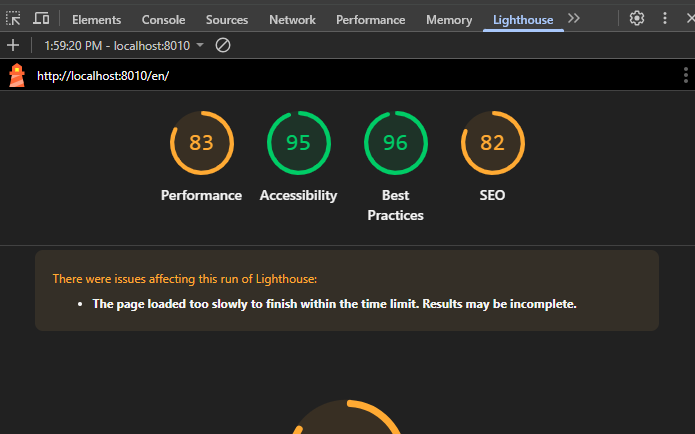
\includegraphics[width=0.7\textwidth]{assets/pics/bab4_navigation.png}
    \caption{Hasil Keseluruhan Pengujian Navigasi}
\end{figure}

Hasil pengujian keseluruhan menunjukkan skor berikut:
\begin{itemize}
    \item Performance: 83
    \item Accessibility: 95
    \item Best Practices: 96
    \item SEO: 82
\end{itemize}

\subsubsection{Performance}
\begin{figure}[H]
    \centering
    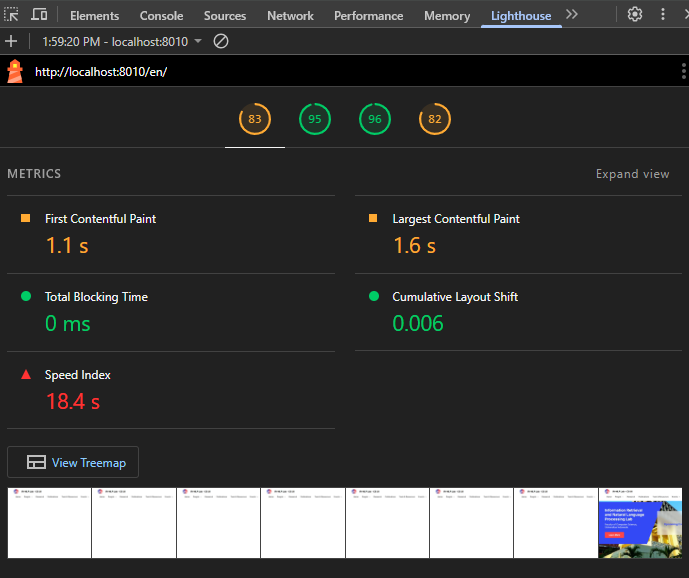
\includegraphics[width=0.7\textwidth]{assets/pics/bab4_performance.png}
    \caption{Hasil Pengujian Performa}
\end{figure}

Website memperoleh nilai performa sebesar 83 yang menunjukkan bahwa performa website berada dalam kategori baik. Beberapa metrik utama yang diukur pada pengujian ini adalah sebagai berikut:

\begin{itemize}
    \item Largest Contentful Paint (LCP): 1.6 detik
    \item Total Blocking Time (TBT): 0 ms
    \item First Contentful Paint (FCP): 1.1 detik
    \item Cumulative Layout Shift (CLS): 0.006
    \item Speed Index: 1.84 detik
\end{itemize}

Lighthouse juga memberikan beberapa rekomendasi optimasi performa sebagai berikut:

\begin{figure}[H]
    \centering
    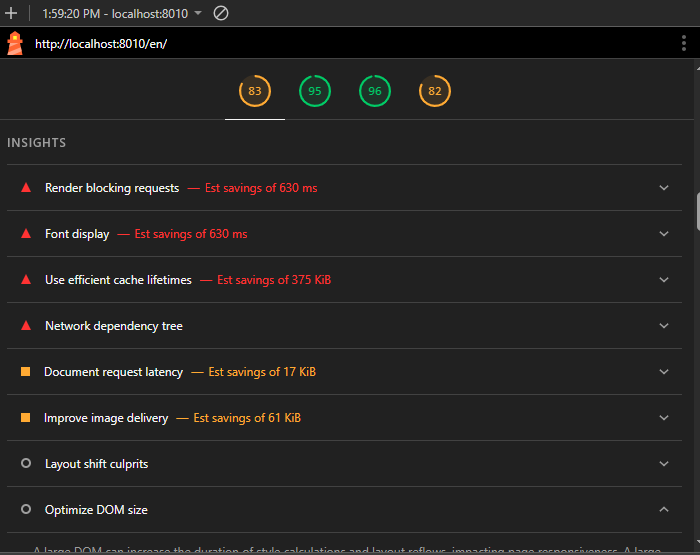
\includegraphics[width=0.7\textwidth]{assets/pics/bab4_performance_recomendation.png}
    \caption{Rekomendasi Optimasi Performa}
\end{figure}

Rekomendasi utama yang diberikan adalah mengoptimalkan ukuran gambar, yaitu dengan menyesuaikan ukuran gambar asli agar sesuai dengan ukuran tampilan pada website. Hal ini bertujuan untuk mengurangi beban pemuatan halaman.

\subsubsection{Accessibility}
\begin{figure}[H]
    \centering
    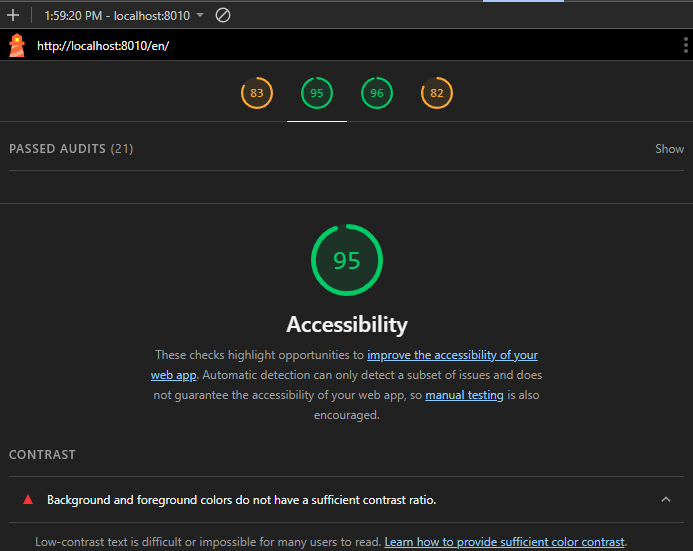
\includegraphics[width=0.7\textwidth]{assets/pics/bab4_accesibility.png}
    \caption{Hasil Pengujian Accessibility}
\end{figure}

Website memperoleh nilai Accessibility sebesar 95 yang menunjukkan bahwa tingkat aksesibilitas website berada dalam kategori sangat baik. Meskipun demikian, Lighthouse memberikan satu rekomendasi, yaitu penggunaan warna teks putih di atas latar belakang berwarna merah dapat mengurangi tingkat kontras, sehingga berpotensi menyulitkan pengguna dengan gangguan penglihatan.

\begin{figure}[H]
    \centering
    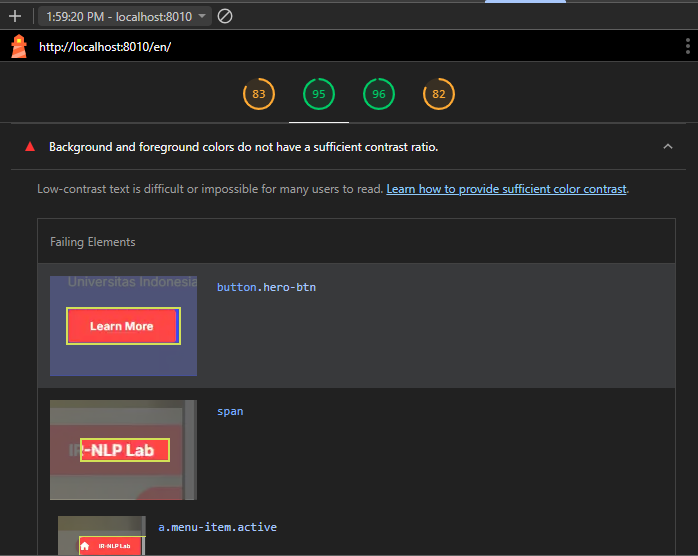
\includegraphics[width=0.7\textwidth]{assets/pics/bab4_accesibility_recommendation.png}
    \caption{Rekomendasi Optimasi Accessibility}
\end{figure}

\subsubsection{Best Practices}
\begin{figure}[H]
    \centering
    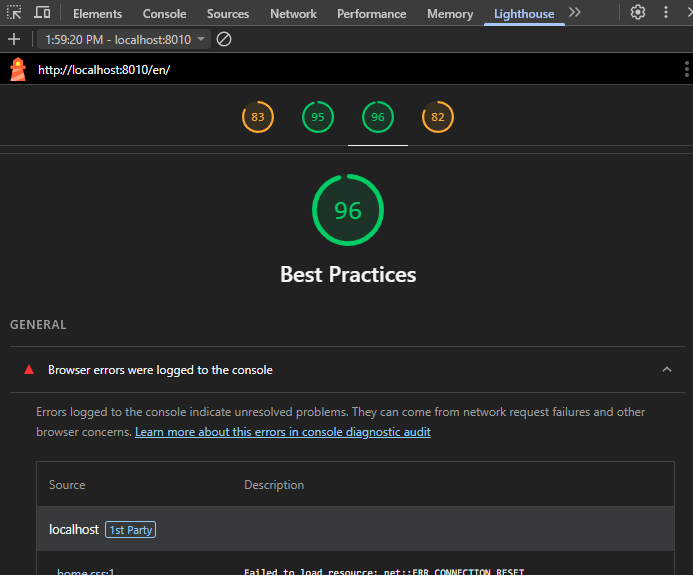
\includegraphics[width=0.7\textwidth]{assets/pics/bab4_bestpractice.png}
    \caption{Hasil Pengujian Best Practices}
\end{figure}

Website memperoleh nilai Best Practices sebesar 96 yang menunjukkan bahwa website telah mengikuti standar praktik terbaik dalam pengembangan web. Hanya terdapat satu rekomendasi yang diberikan, yaitu adanya kesalahan bawaan yang tercatat (logged) pada Console browser.

\subsubsection{SEO}
\begin{figure}[H]
    \centering
    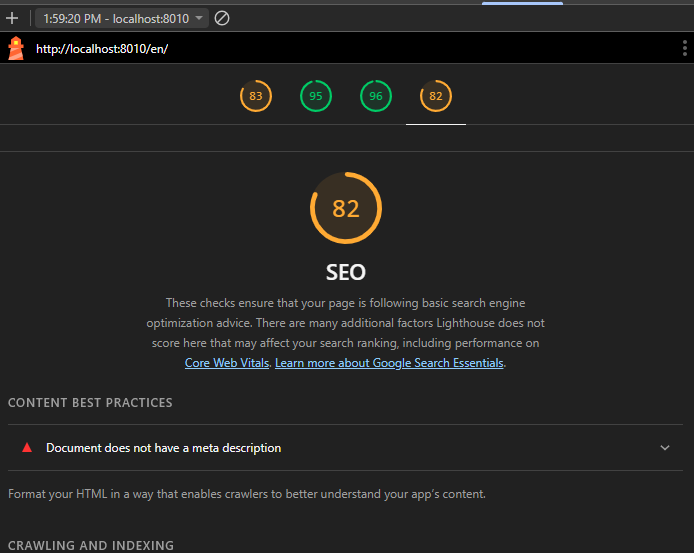
\includegraphics[width=0.7\textwidth]{assets/pics/bab4_seo.png}
    \caption{Hasil Pengujian SEO}
\end{figure}

Website memperoleh nilai SEO sebesar 82 yang menunjukkan bahwa optimasi mesin pencari berada dalam kategori baik. Untuk meningkatkan kualitas SEO, disarankan untuk menambahkan \textit{meta description} pada setiap halaman website.

\subsubsection{Timespan}
\begin{figure}[H]
    \centering
    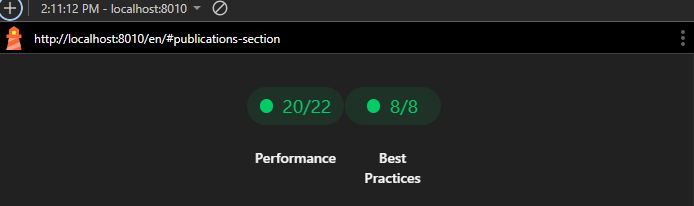
\includegraphics[width=0.7\textwidth]{assets/pics/bab4_timespan.png}
    \caption{Hasil Pengujian Timespan}
\end{figure}

\subsubsection{Timespan Performance}
\begin{figure}[H]
    \centering
    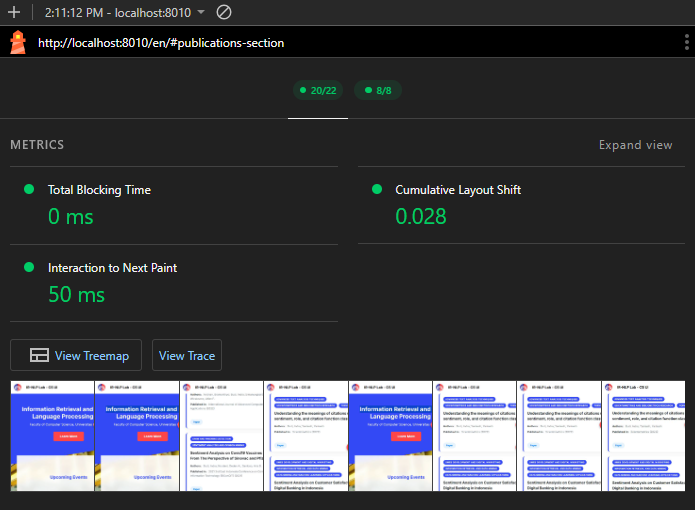
\includegraphics[width=0.7\textwidth]{assets/pics/bab4_timespan_performance_time.png}
    \caption{Hasil Pengujian Timespan Performance Time}
\end{figure}

Website memperoleh nilai performa timespan sebesar 20 dari 22, yang menunjukkan bahwa performa website berada dalam kategori sangat baik, dengan metrik sebagai berikut:

\begin{itemize}
    \item Total Blocking Time: 0 ms
    \item Cumulative Layout Shift (CLS): 0.028
    \item Interaction to Next Paint (INP): 50 ms
\end{itemize}

\subsubsection{Timespan Best Practices}
\begin{figure}[H]
    \centering
    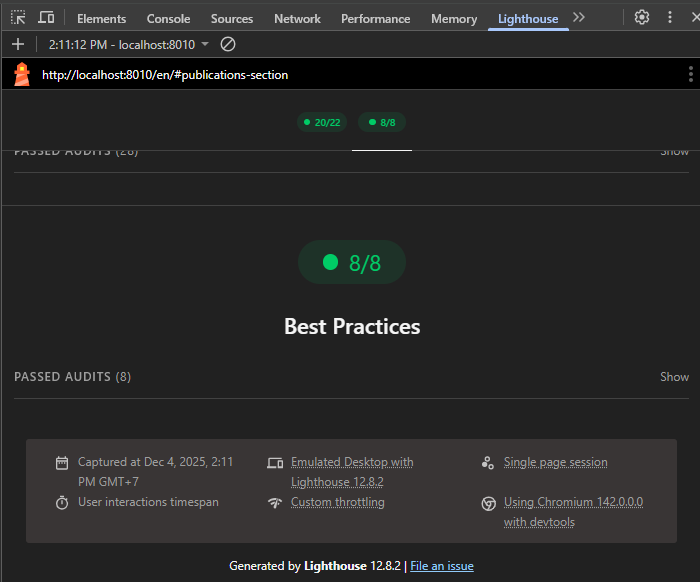
\includegraphics[width=0.7\textwidth]{assets/pics/bab4_timespan_best_practice.png}
    \caption{Hasil Pengujian Timespan Best Practices}
\end{figure}

Pada pengujian Timespan Best Practices, website memperoleh nilai sempurna yaitu 8 dari 8, yang menunjukkan kepatuhan penuh terhadap standar praktik terbaik pada pengujian ini.

\subsection{Pengujian Basis Data}
 Pengujian basis data dilakukan dengan menggunakan django TestCase dilakukan dengan cara mengetes memasukkan data ke database sesuai dengan atribut dari Model
 dan juga pengetesan relasi antar tabel dan juga validasi publikasi.
\begin{figure}[H]
    \centering
    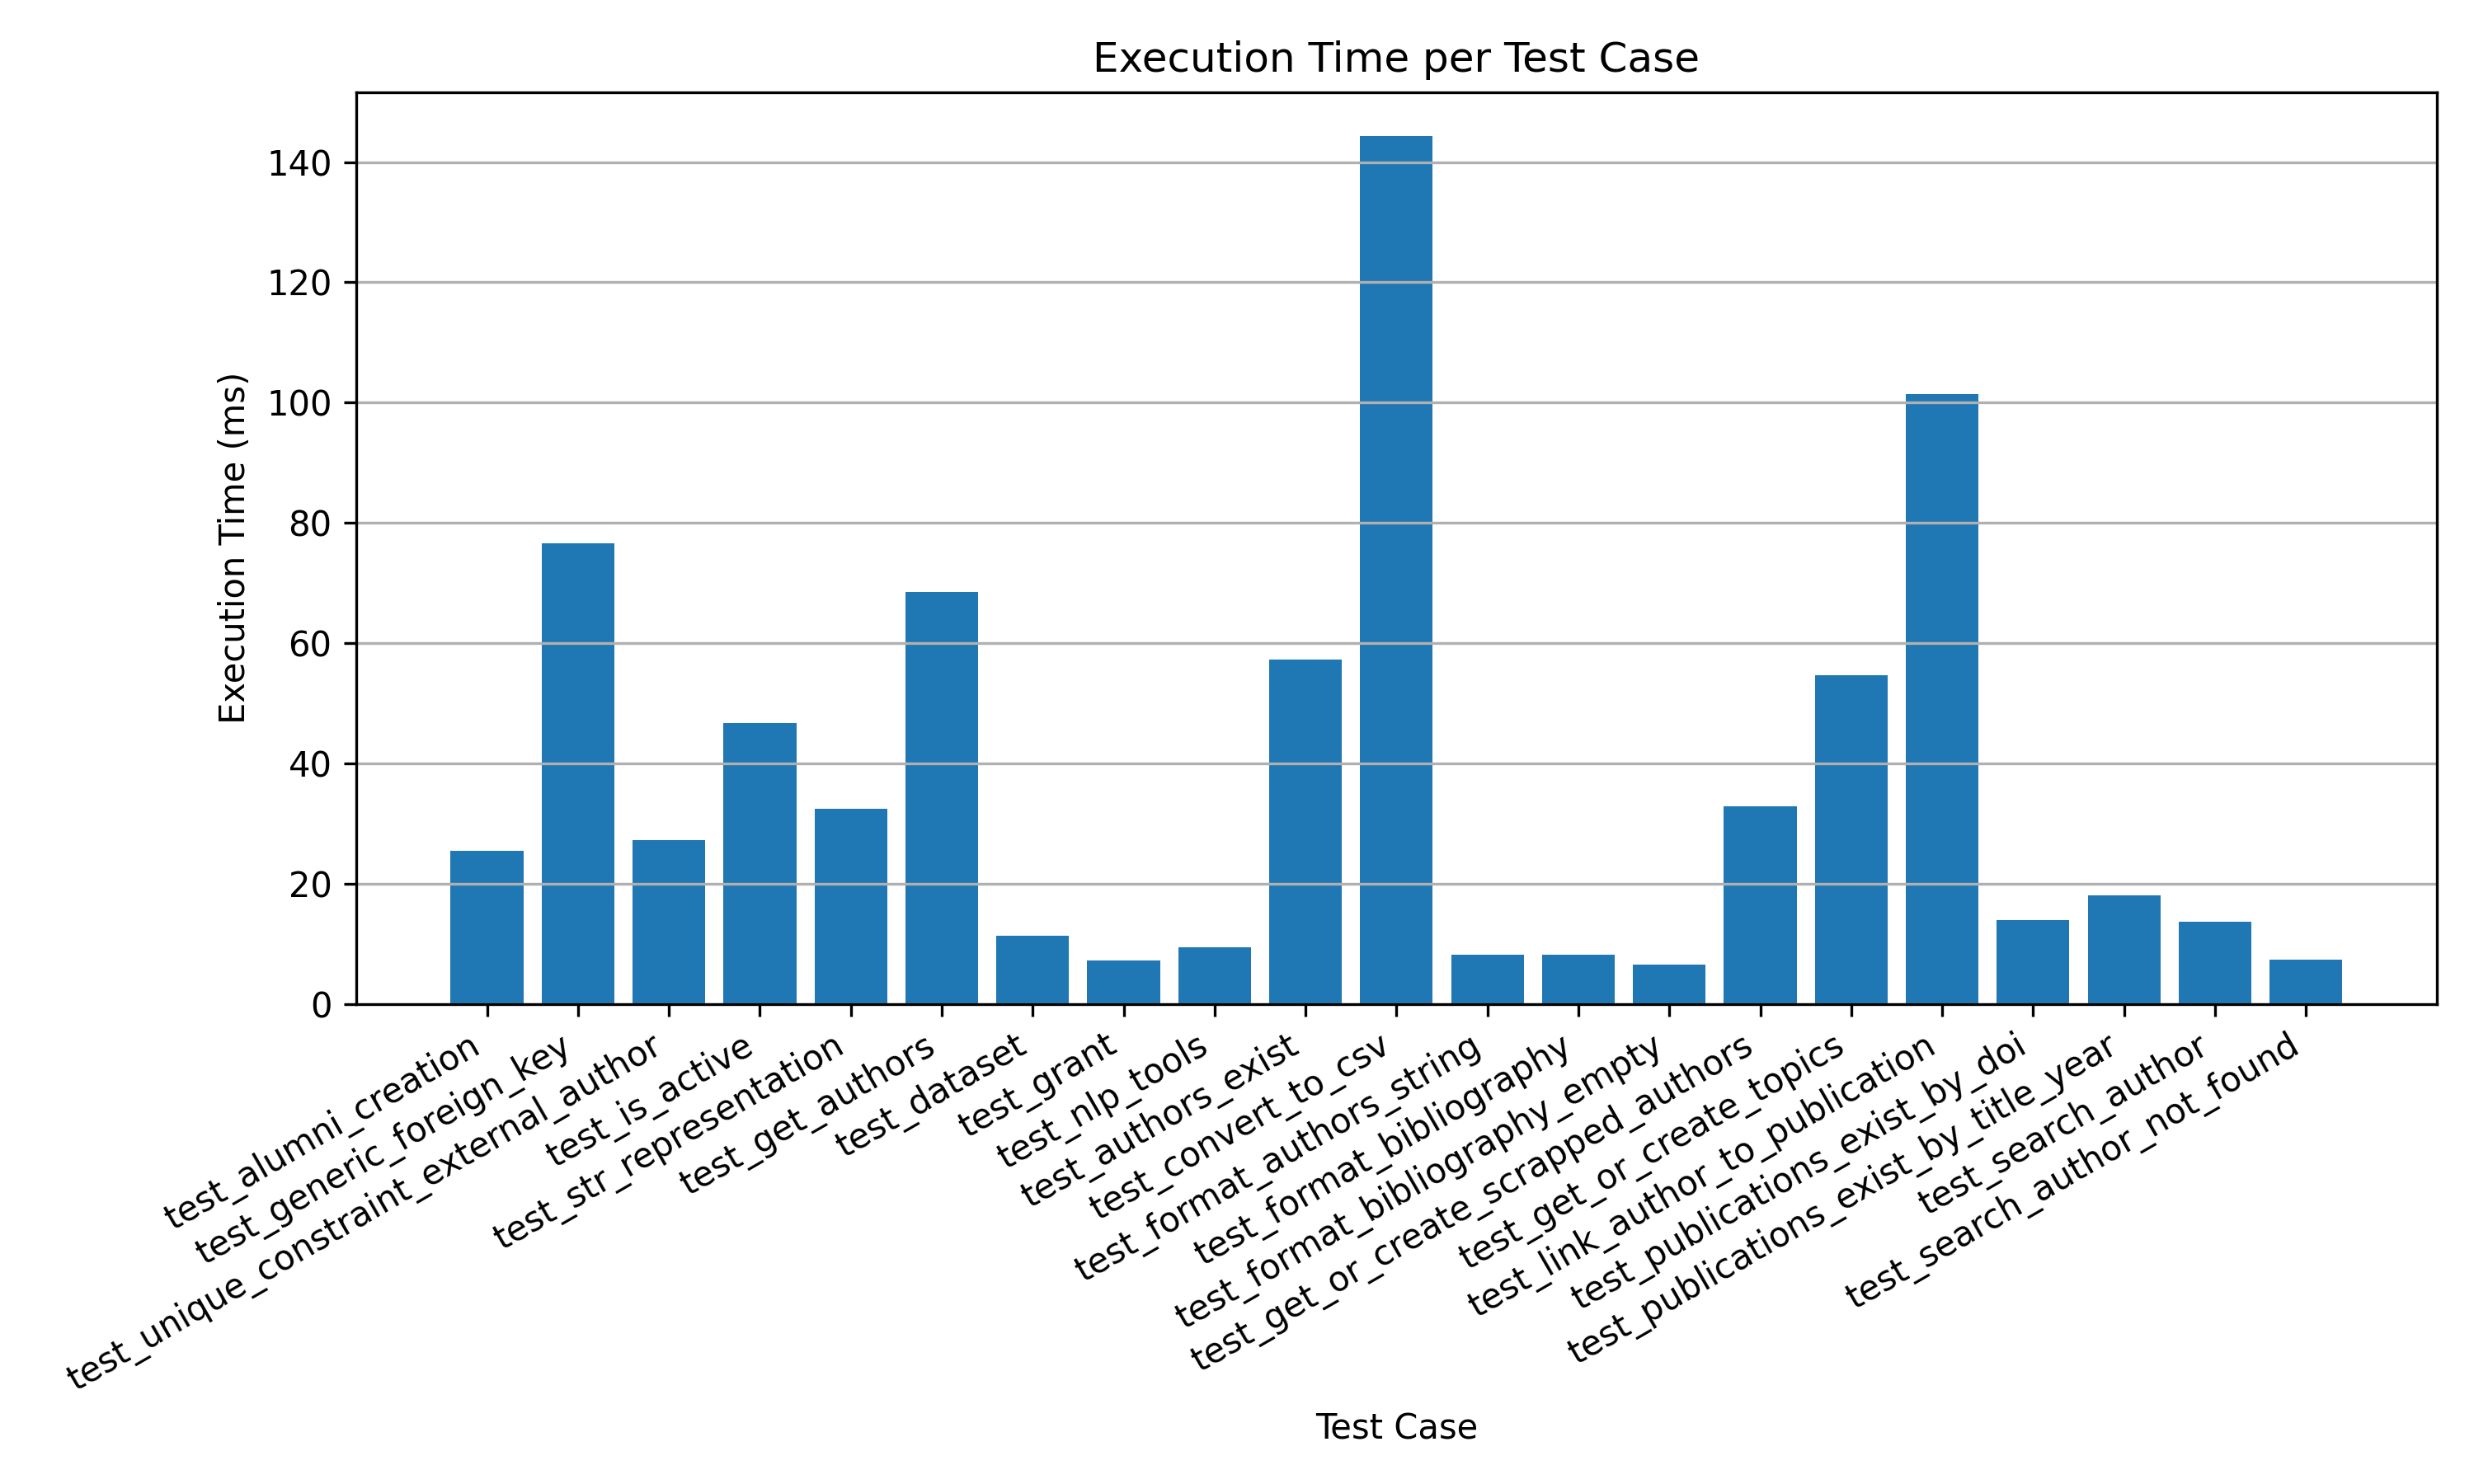
\includegraphics[width=0.7\textwidth]{assets/pics/bab4_bar_execution_time_database.png}
    \caption{Hasil Pengujian Basiss Data berdasarkan waktu eksekusi}
\end{figure}
Ini adalah hasil pengujian bar chart dari waktu eksekusi pengujian basis data. Setiap pengujian dilakukan untuk setiap model yang ada pada sistem, yaitu Model Publication, Event, Tool, Research Group, Member, dan News.
Dari sini dapat dilihat bahwa semua pengujian memiliki waktu eksekusi yang singkat yaitu kurang dari 0.01 detik, yang menandakan bahwa operasi basis data berjalan dengan efisien dan sesuai dengan rancangan sistem.

\begin{figure}[H]
    \centering
    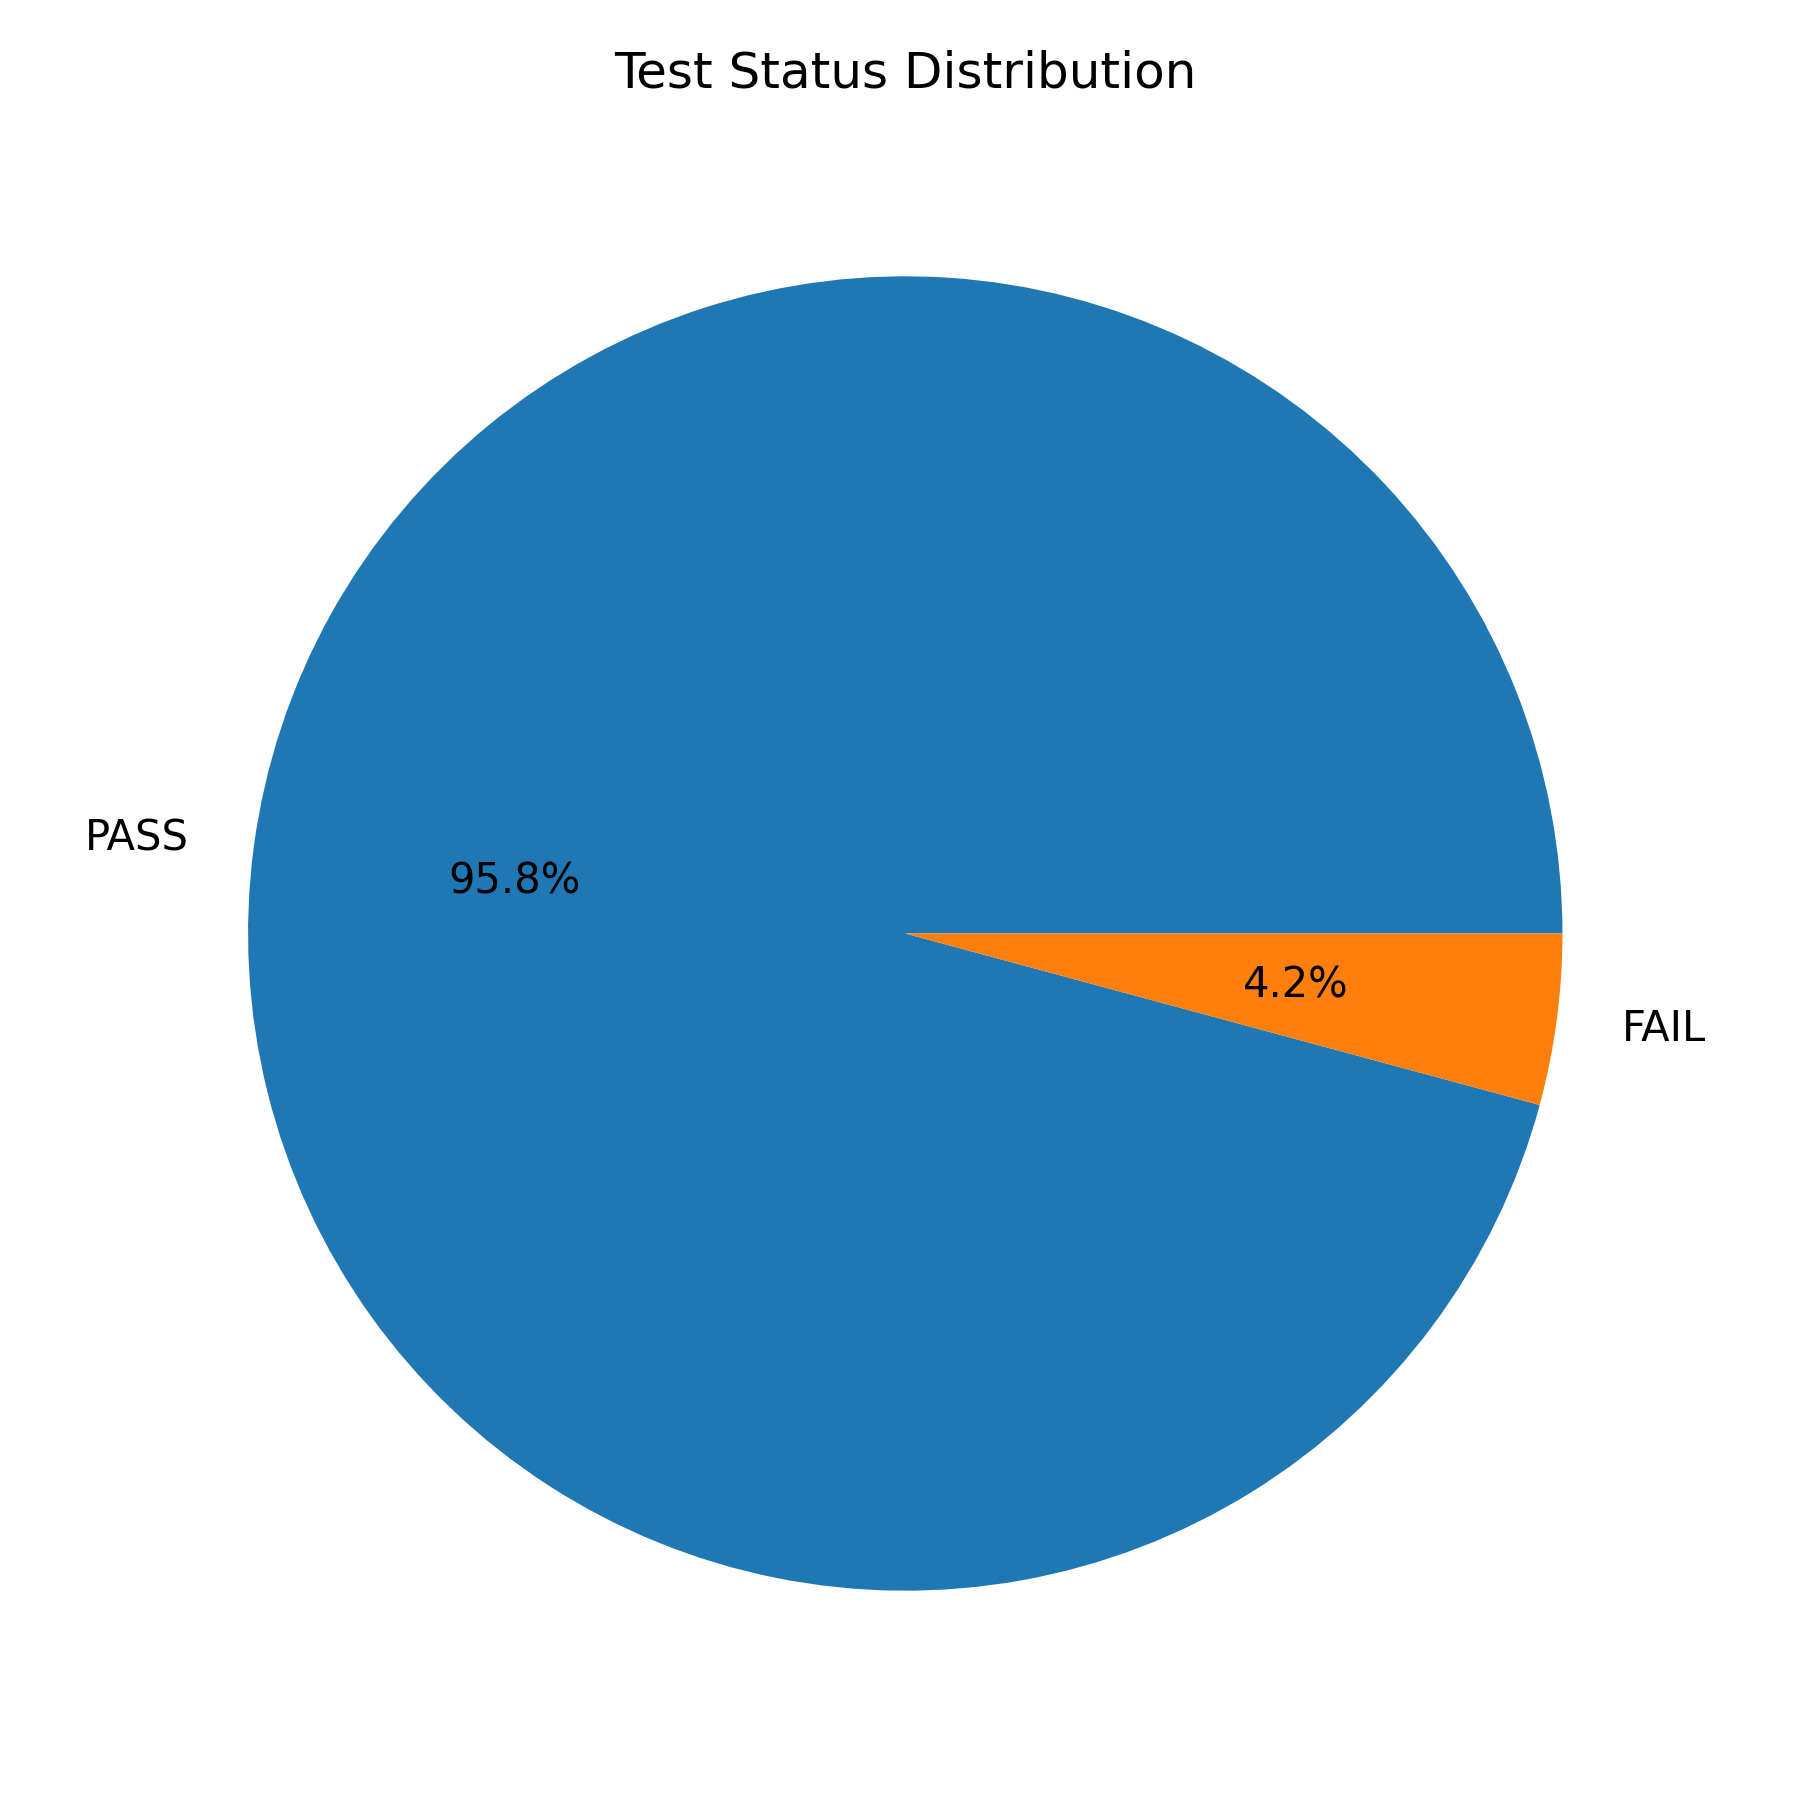
\includegraphics[width=0.7\textwidth]{assets/pics/bab4_pie_test_status_database.png}
    \caption{Hasil Pengujian Basiss Data berdasarkan status pengujian}
\end{figure}

Ini adalah hasil piechart dari status pengujian basis data. Ada sebagian kecil pengujian yang gagal dan hasilnya 

\begin{figure}[H]
    \centering
    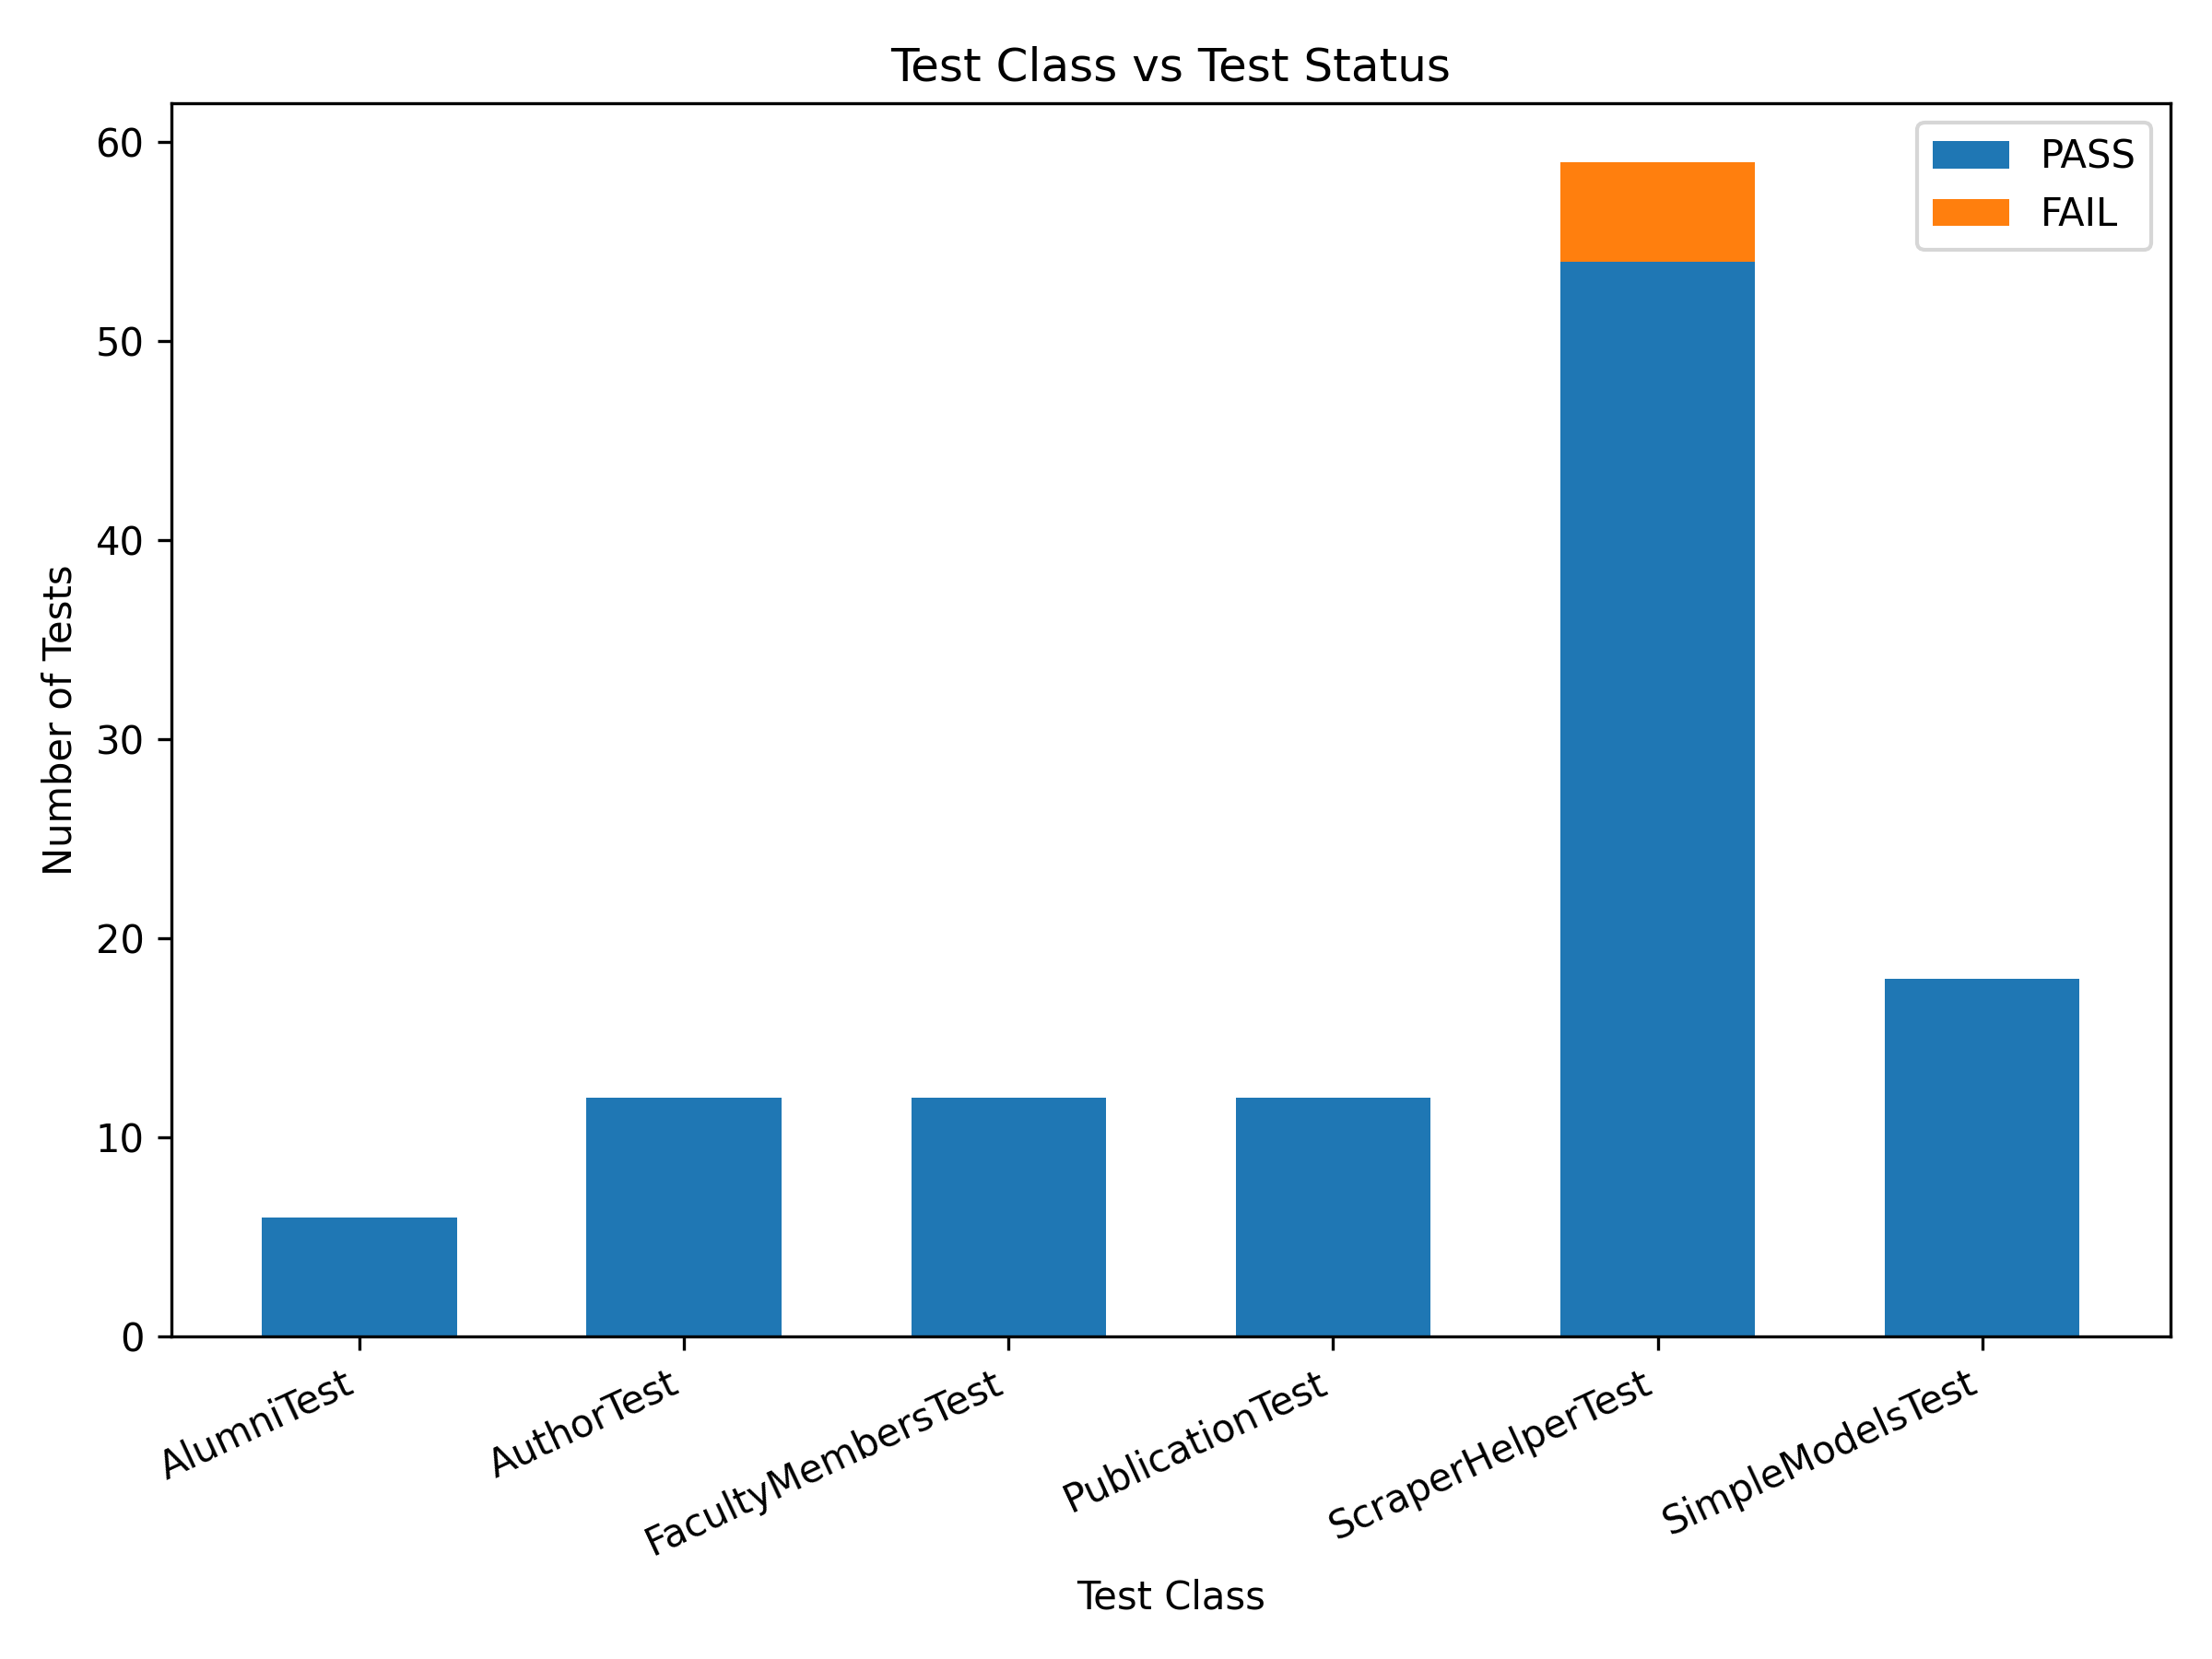
\includegraphics[width=0.7\textwidth]{assets/pics/bab4_stacked_test_class_status_database.png}
    \caption{Hasil Pengujian Basis Data berdasarkan kelas pengujian}
\end{figure}

Ini adalah stacked bar chart dari status pengujian berdasarkan kelas pengujian. Setiap kelas pengujian mewakili model yang ada pada sistem. Dari sini dapat dilihat bahwa Seluruh kelas basis data memiliki status pengujian yang berhasil, hanya ada sedikit gagal pada kelas Publikasi Scraper namun seluruhnya telah diperbaiki

\begin{figure}[H]
    \centering
    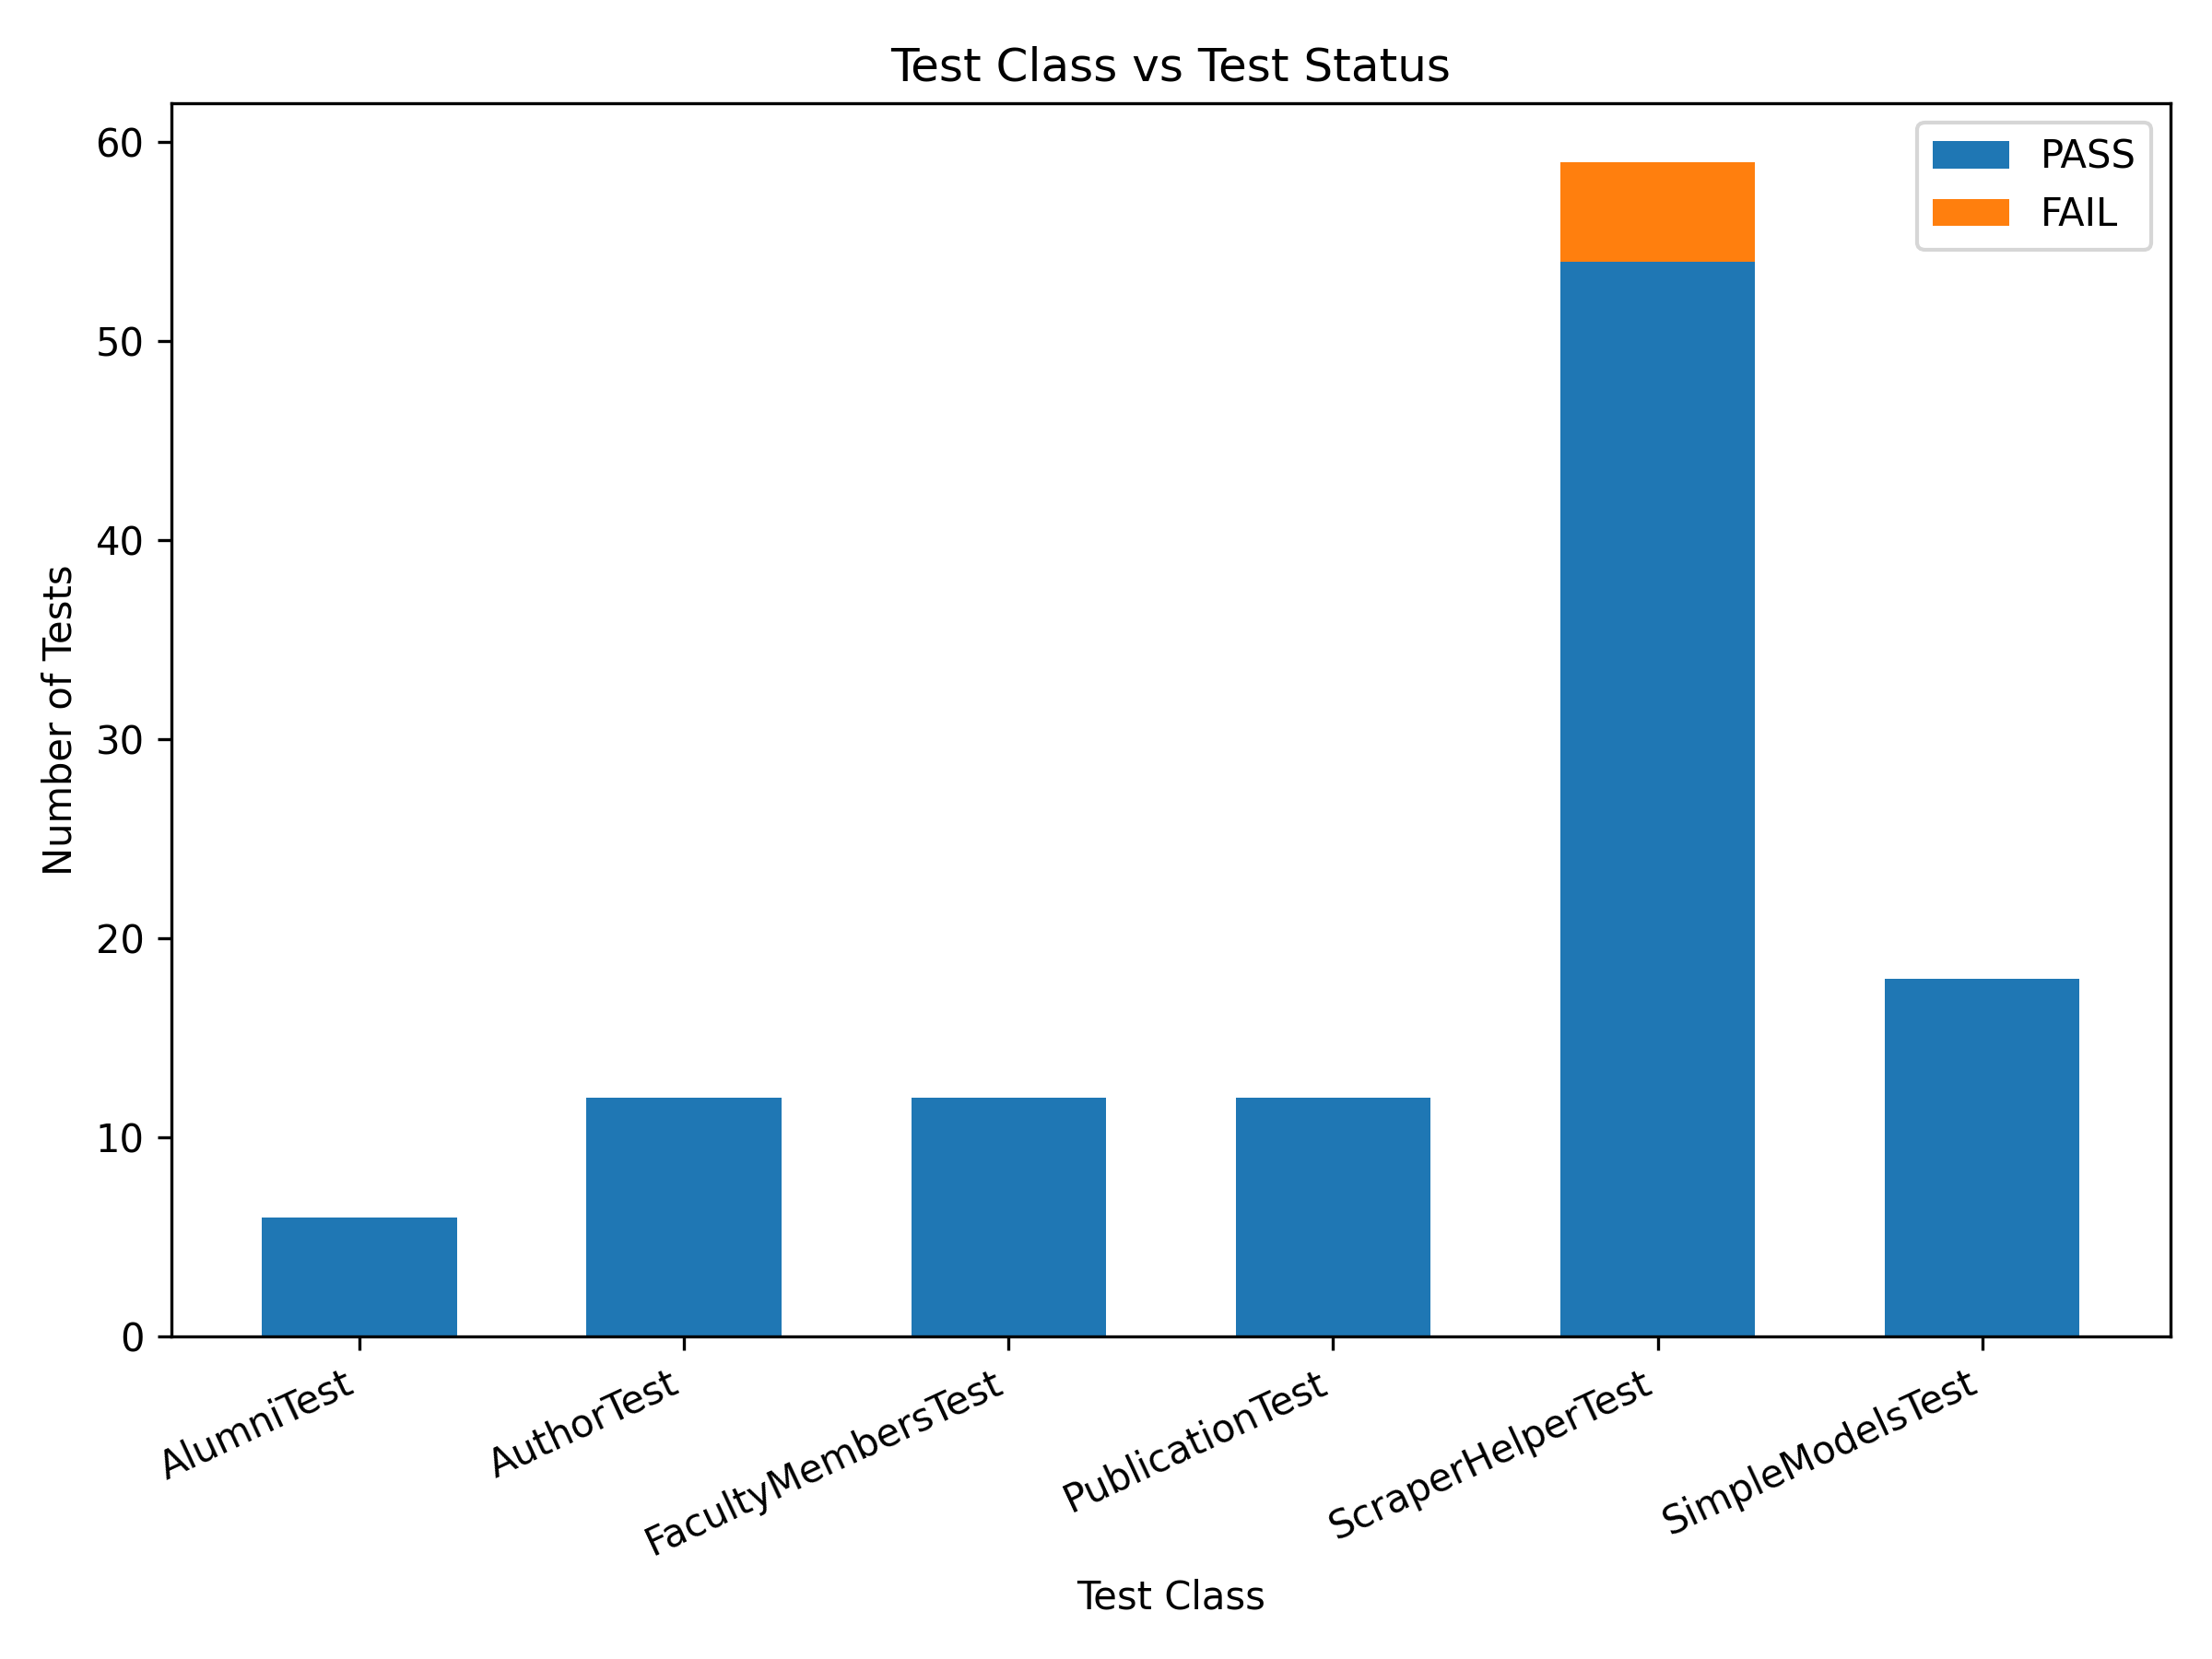
\includegraphics[width=0.7\textwidth]{assets/pics/bab4_stacked_test_class_status_database.png}
    \caption{Hasil Pengujian Basis Data berdasarkan waktu dilakukan pengujian}
\end{figure}

Ini adalah timeline dari pengujian basis data berdasarkan data tersebut pengujian dilakukan beberapa kali dari jam 11:30 hingga 13:45 dengan diantara waktu dilakukan perbaikian pada pengujian yang berhasal
dapat dilihat bahwa awal pengujian sedikit namun ditingkatkan selanjutnya dengan menambahkan pengujian dan seiring pengujian kegagalan test diperbaiki

\subsection{Pengujian View}
Pengujian Views dilakukan dengan menggunakan django TestCase dilakukan dengan cara mengetes setiap URL yang ada pada sistem apakah dapat diakses dengan benar dan juga memastikan bahwa setiap view mengembalikan response yang sesuai seperti 200 OK atau 302
\begin{figure}[H]
    \centering
    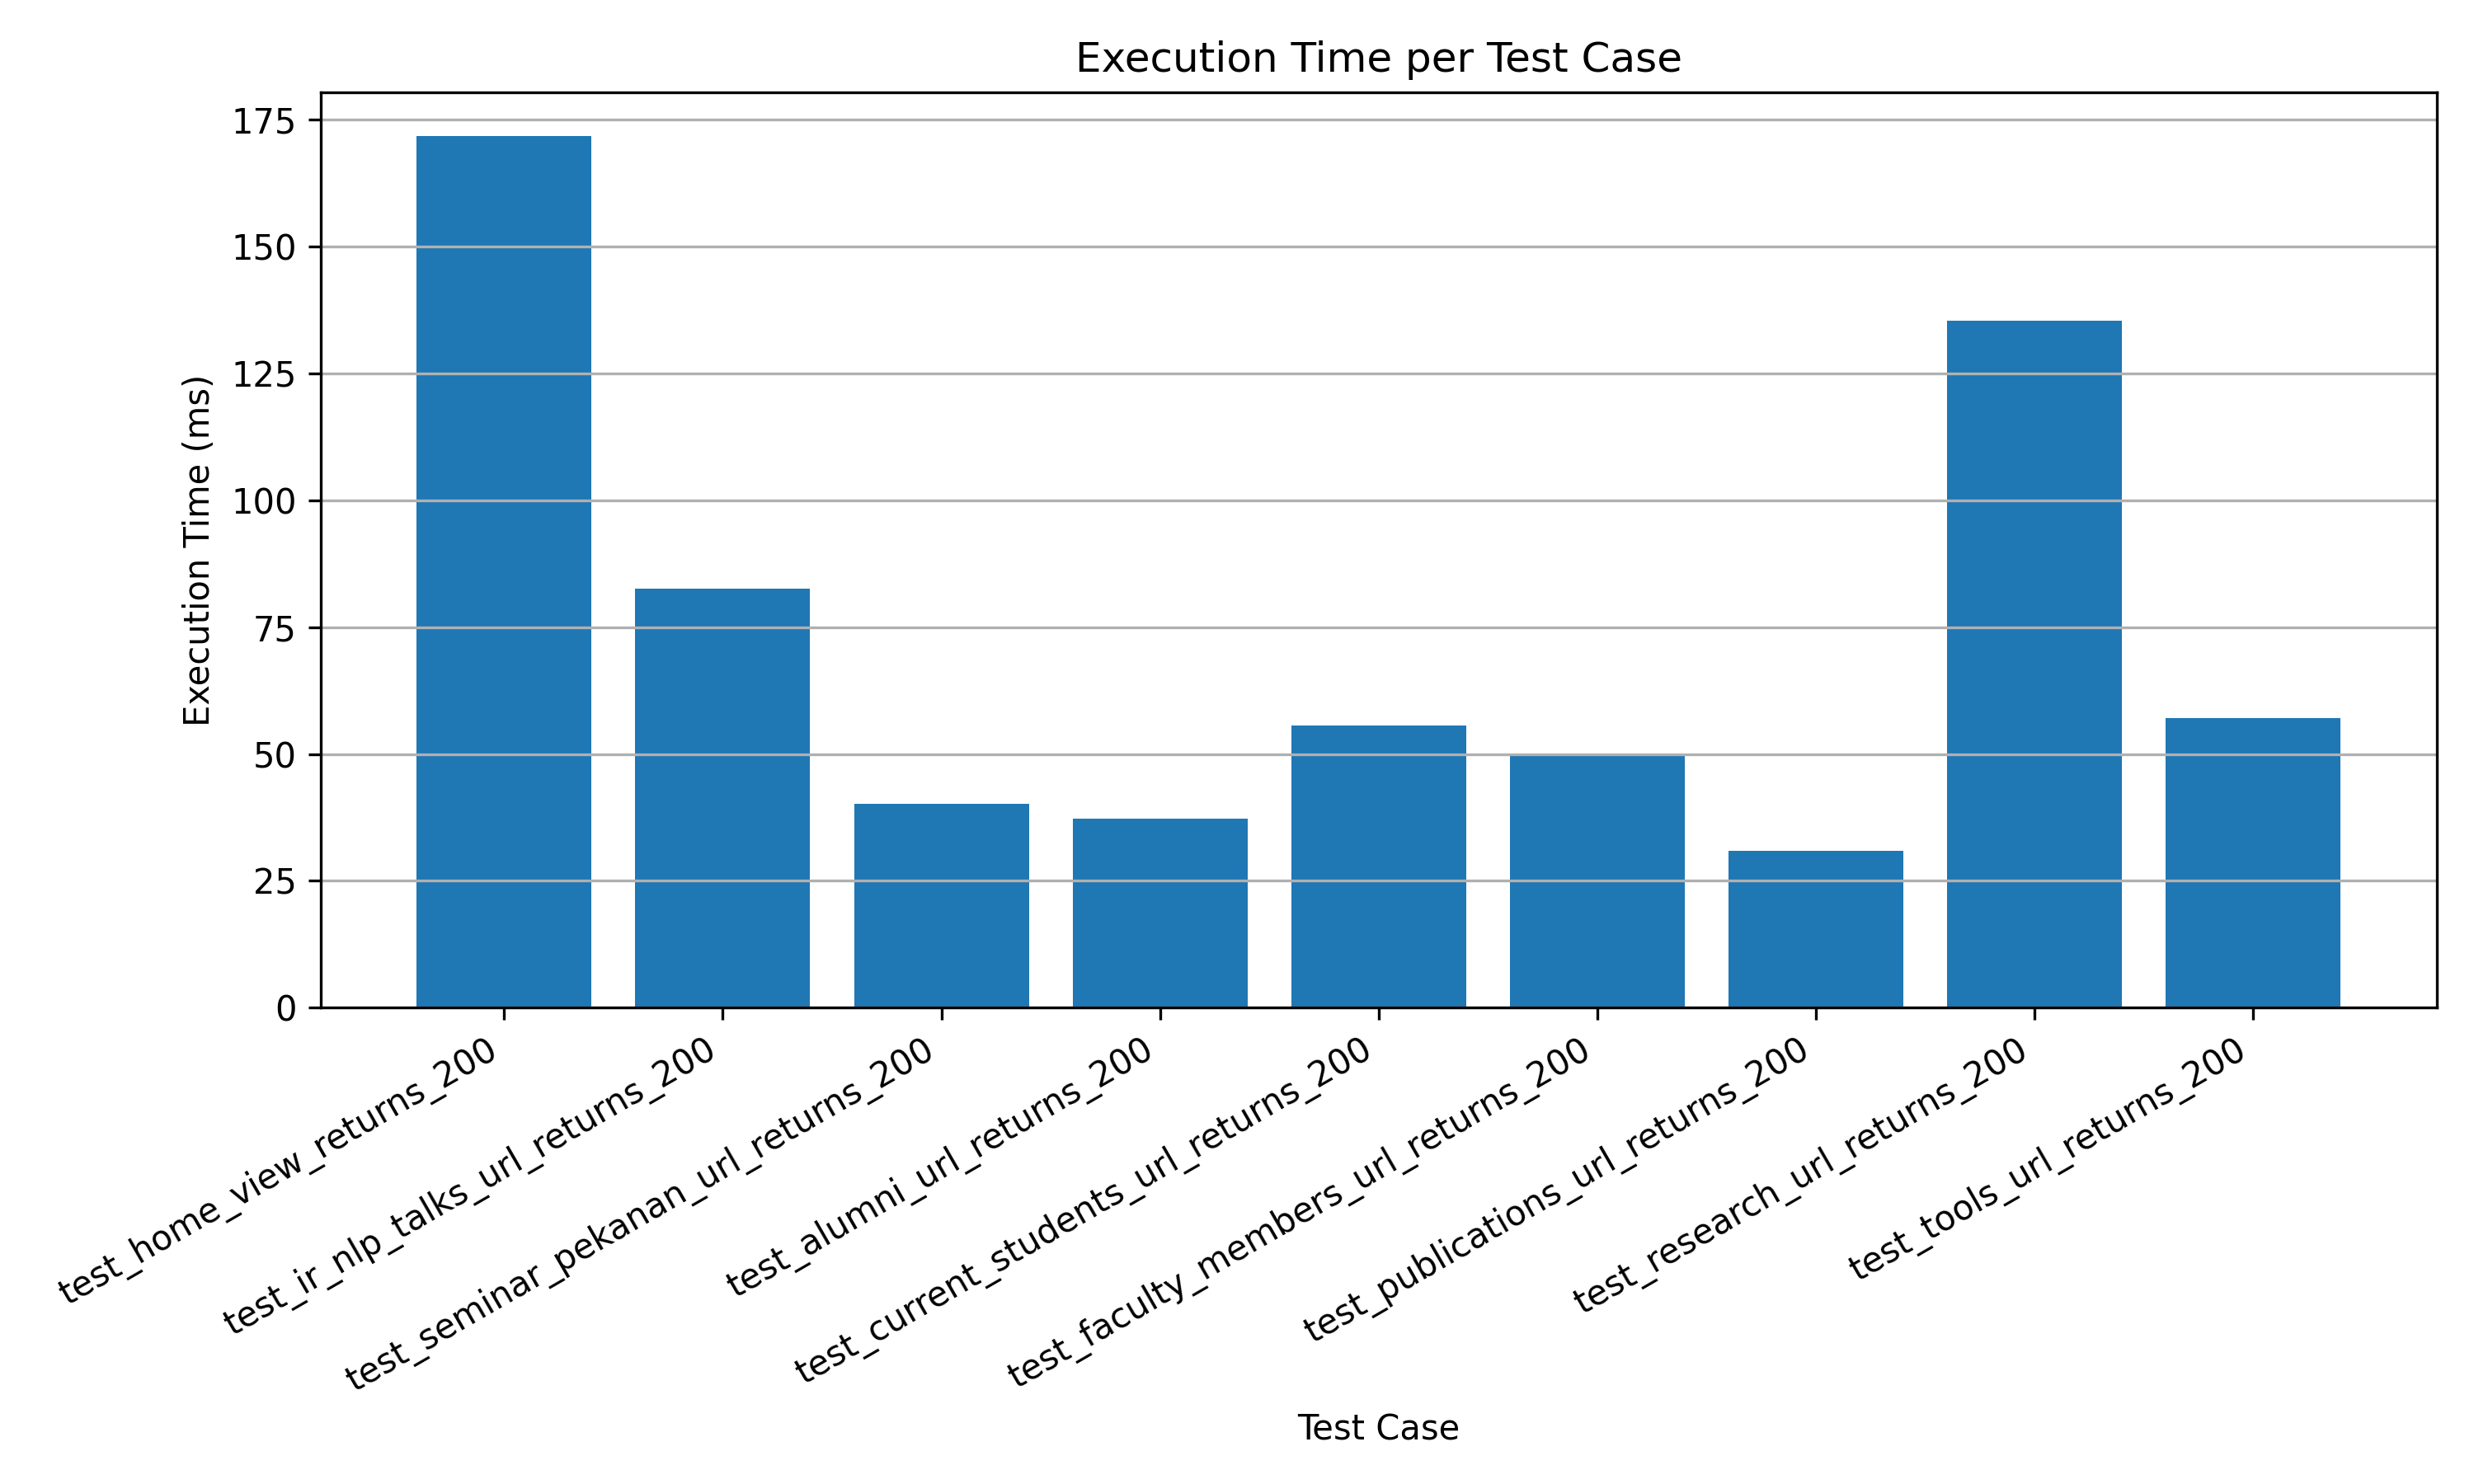
\includegraphics[width=0.7\textwidth]{assets/pics/bab4_bar_execution_time_views.png}
    \caption{Hasil Pengujian Views berdasarkan waktu eksekusi}
\end{figure}
Ini adalah hasil pengujian bar chart dari waktu eksekusi pengujian views. Setiap pengujian dilakukan untuk setiap URL yang ada pada sistem.
Dari sini dapat dilihat bahwa semua pengujian memiliki waktu eksekusi yang singkat yaitu kurang dari 0.01 detik, yang menandakan bahwa operasi views berjalan dengan efisien dan sesuai dengan rancangan sistem.
\begin{figure}[H]
    \centering
    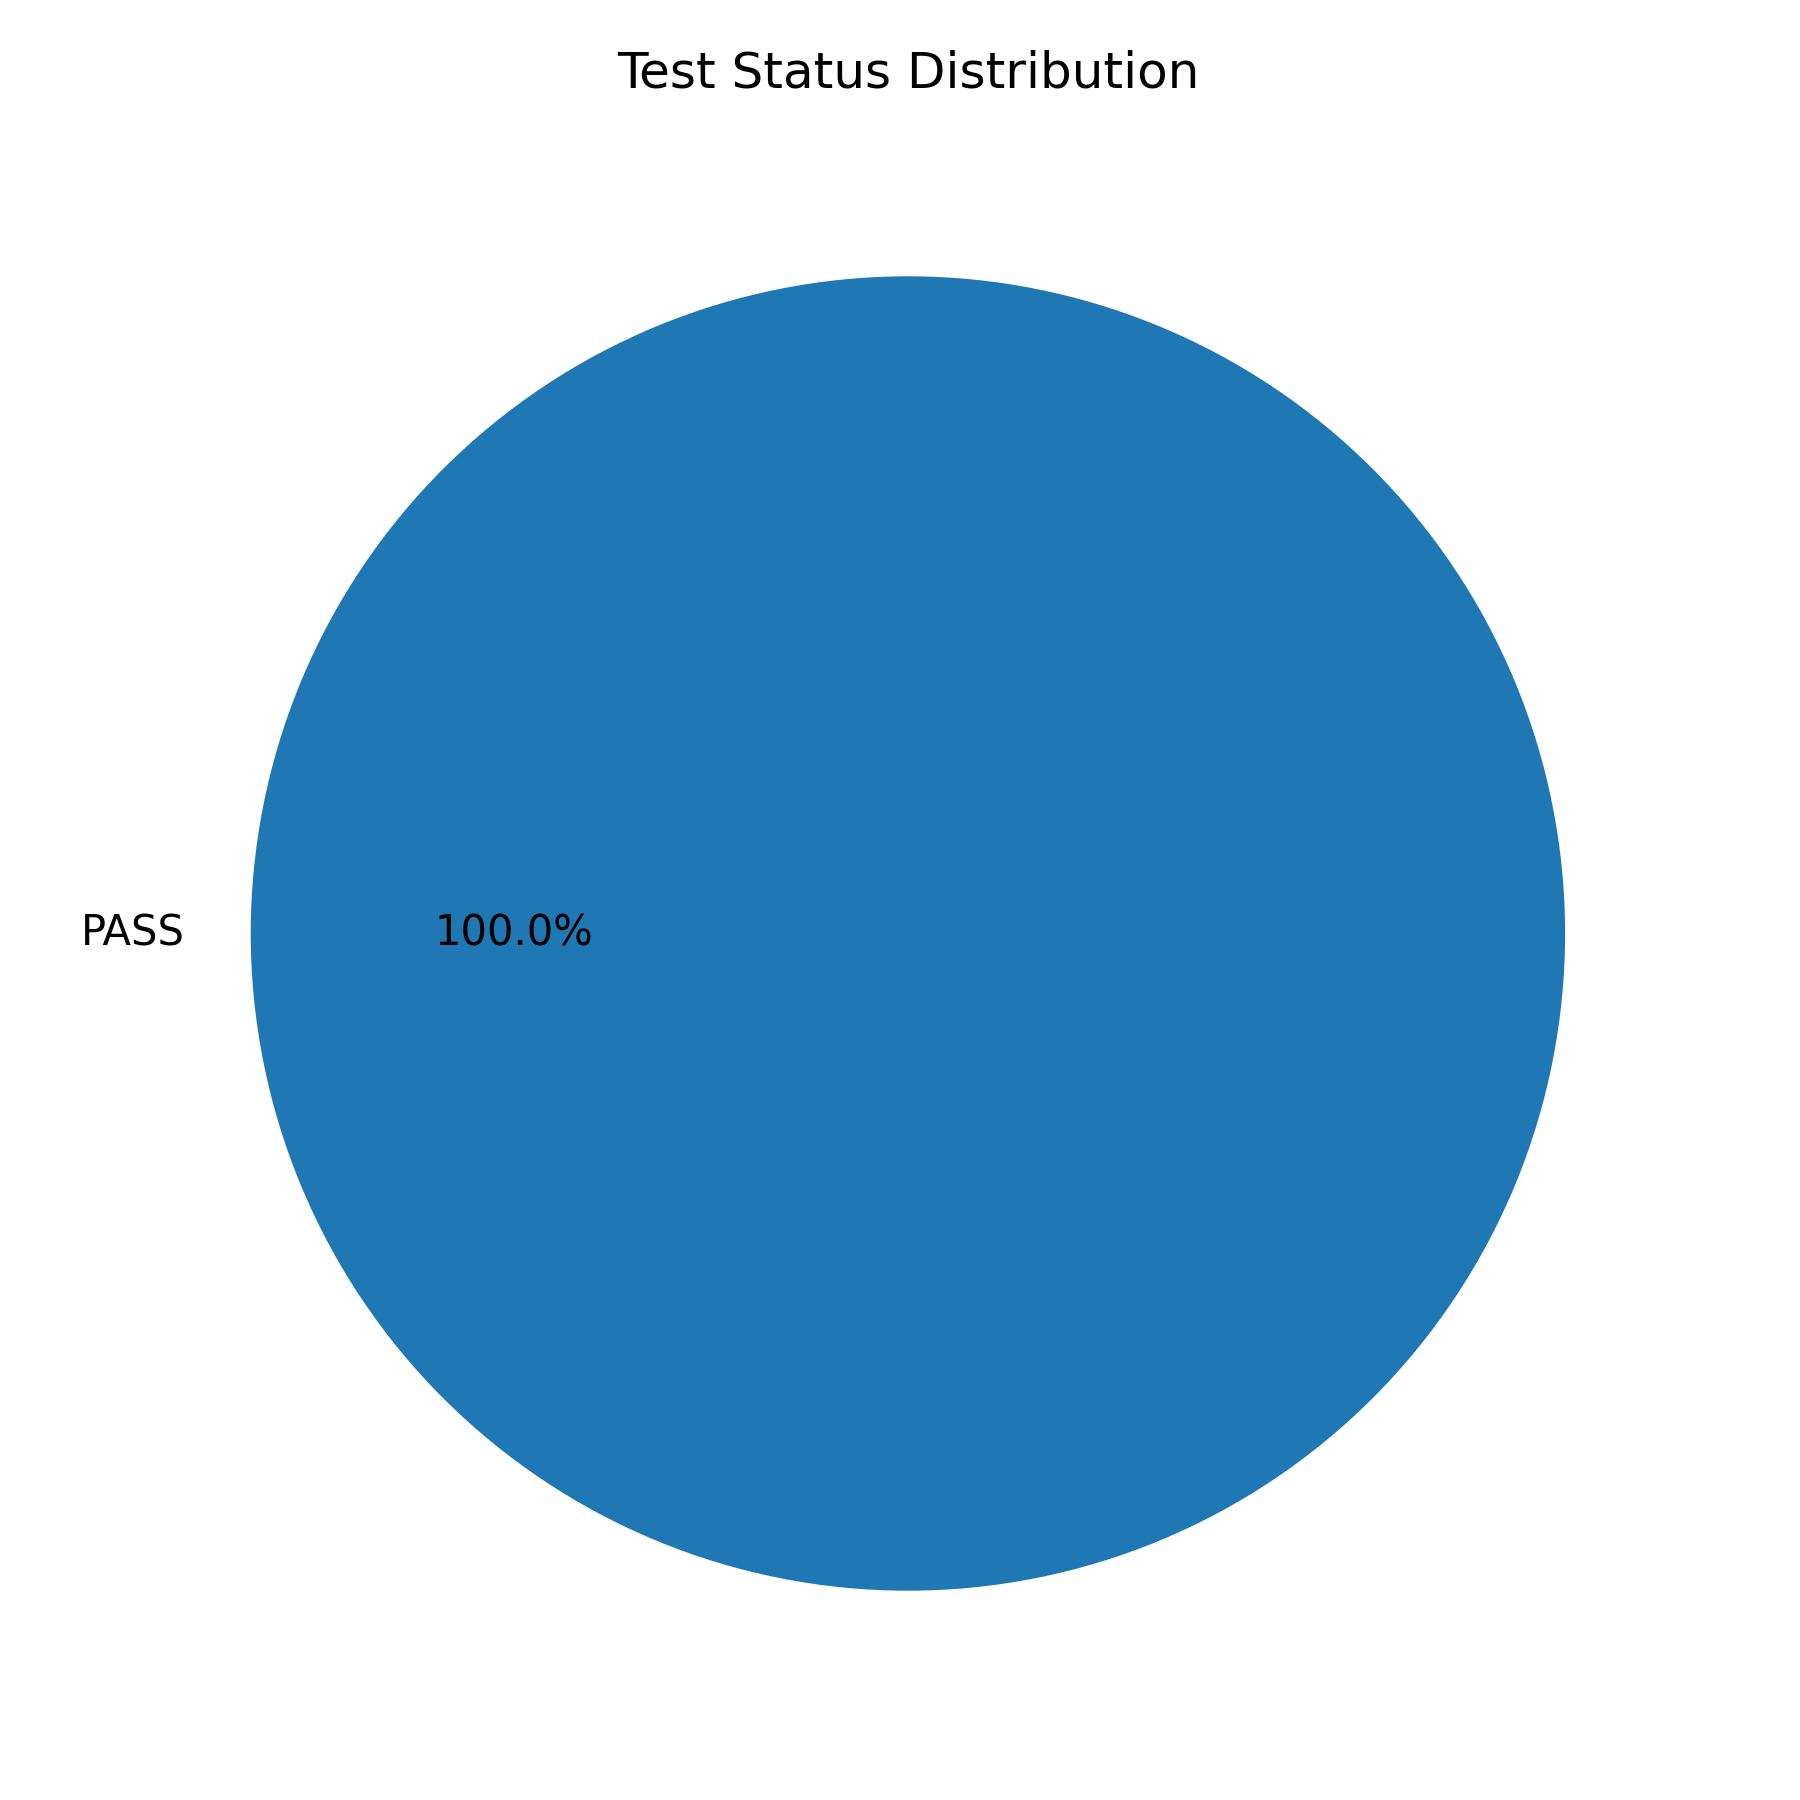
\includegraphics[width=0.7\textwidth]{assets/pics/bab4_pie_test_status_views.png}
    \caption{Hasil Pengujian Views berdasarkan status pengujian}
\end{figure}

Ini adalah hasil piechart dari status pengujian views. Ada sebagian kecil pengujian yang gagal dan hasilnya 

\begin{figure}[H]
    \centering
    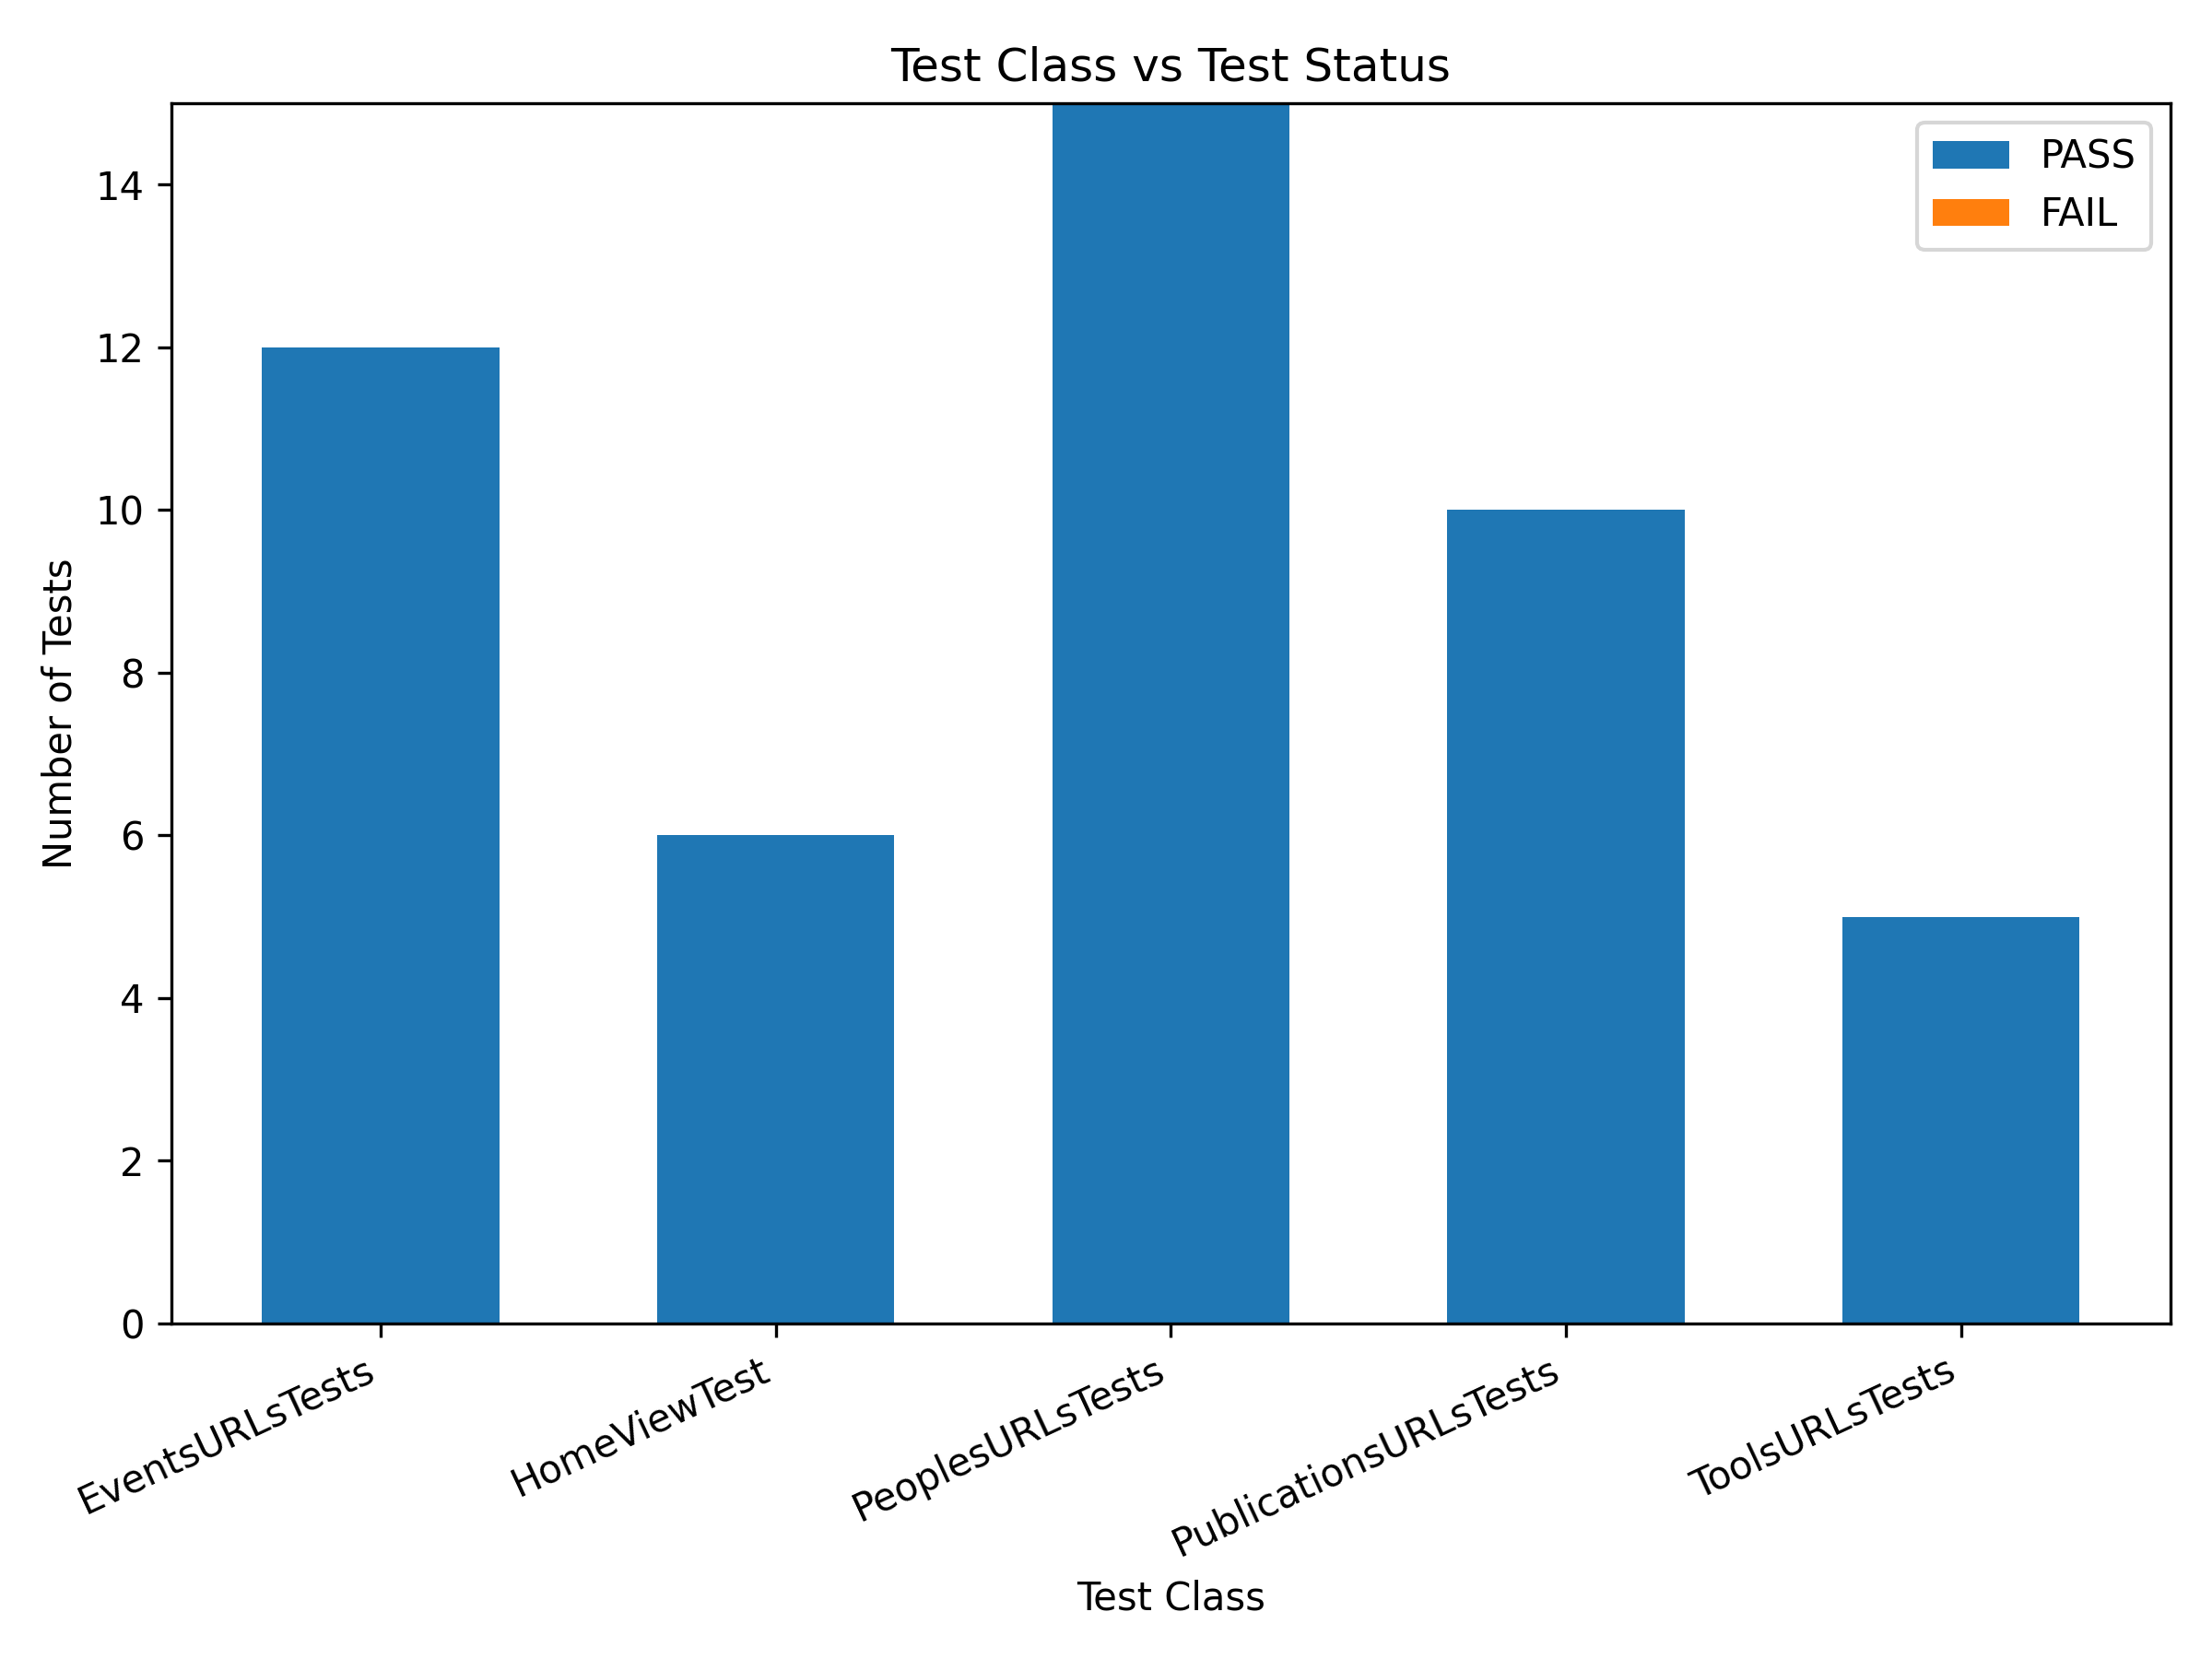
\includegraphics[width=0.7\textwidth]{assets/pics/bab4_stacked_test_class_status_views.png}
    \caption{Hasil Pengujian Views berdasarkan kelas pengujian}
\end{figure}

Ini adalah stacked bar chart dari status pengujian berdasarkan kelas pengujian. Setiap kelas pengujian mewakili model yang ada pada sistem. Dari sini dapat dilihat bahwa Seluruh kelas basis data memiliki status pengujian yang berhasil, hanya ada sedikit gagal pada kelas Publikasi Scraper namun seluruhnya telah diperbaiki

\begin{figure}[H]
    \centering
    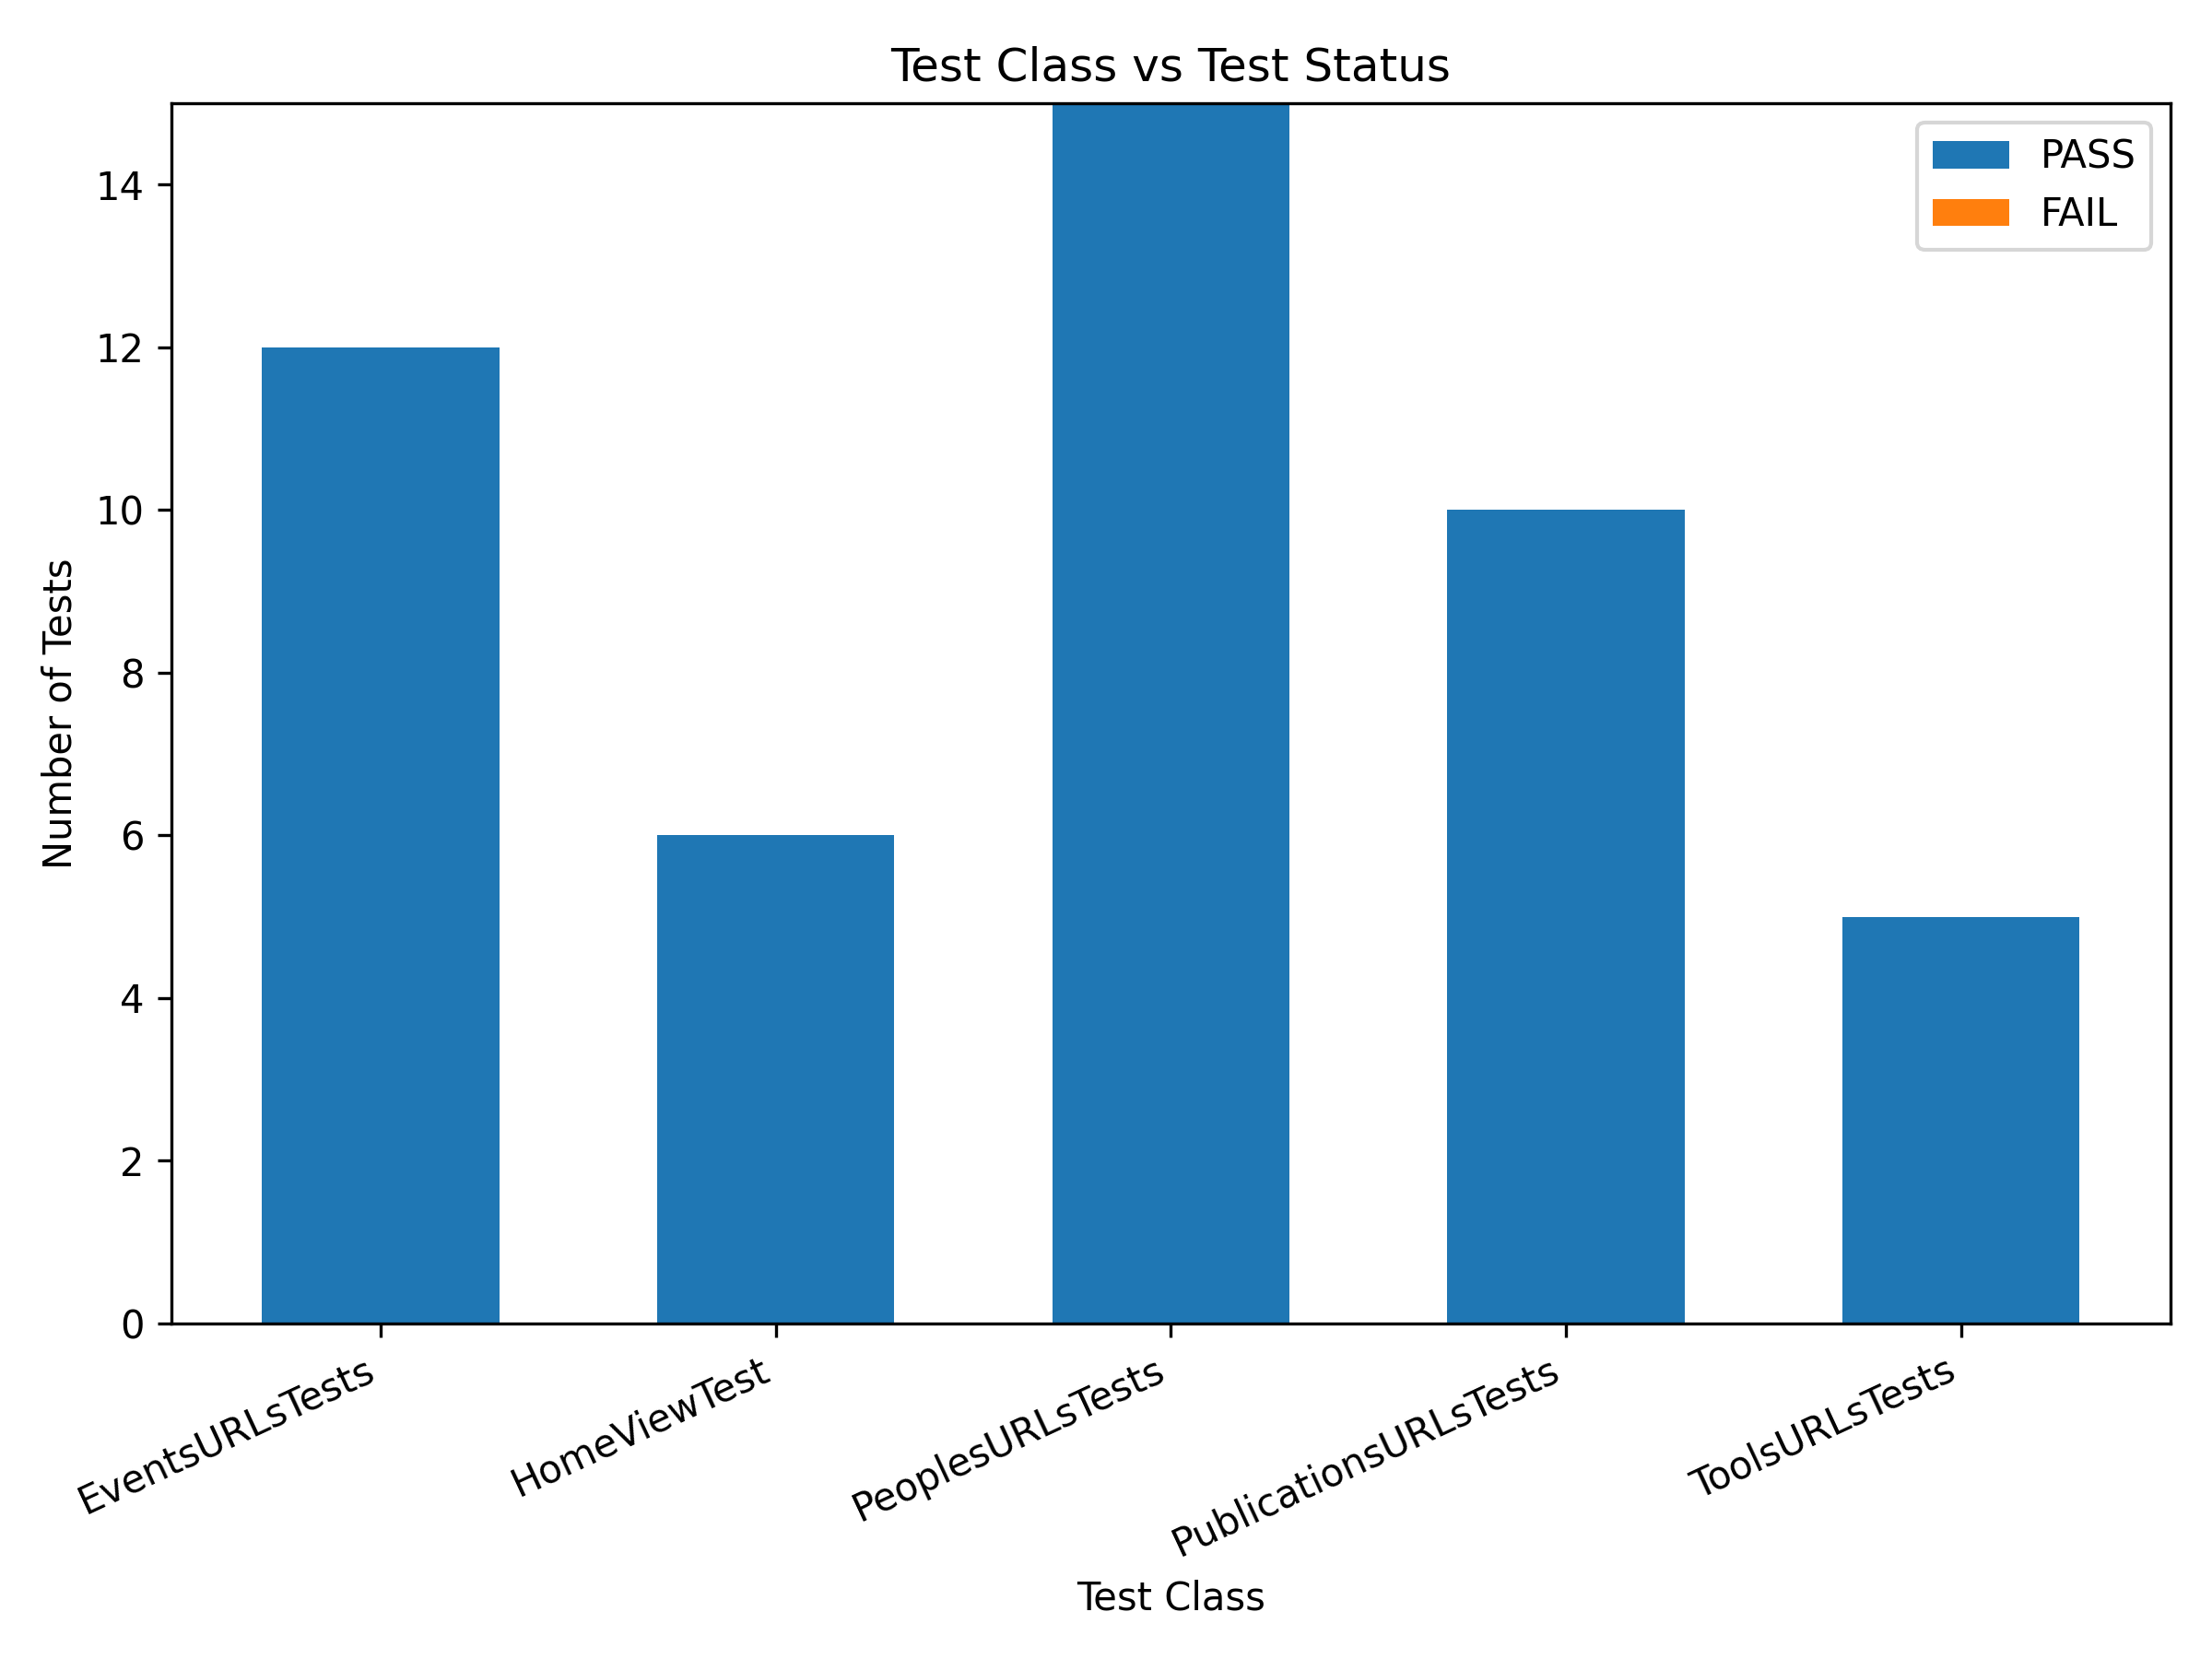
\includegraphics[width=0.7\textwidth]{assets/pics/bab4_stacked_test_class_status_views.png}
    \caption{Hasil Pengujian Views berdasarkan waktu dilakukan pengujian}
\end{figure}

Ini adalah timeline dari pengujian views berdasarkan data tersebut pengujian dilakukan beberapa kali dari jam 11:30 hingga 13:45 dan hasilnya seluruh pengujian berhasil



